
\chapter{Modeling Mass Protest Adoption in Social Network Communities using Geometric Brownian Motion}
%Event Prediction based on Information Propagation\\

% if you want to define paper specific  macros
% then put everthing between begingroup and endgroup
\begingroup
\newcommand{\score}{S}
\newcommand{\myalgo}{CoolAlgo}

%\begin{abstract}
%Modeling the movement of information within social media outlets, like
%Twitter, is key to understanding to how ideas spread but quantifying such
%movement runs into several difficulties. Two specific areas that elude a clear
%characterization are (i) the intrinsic random nature of individuals to
%potentially adopt and subsequently broadcast a Twitter topic, and (ii) the
%dissemination of information via non-Twitter sources, such as news outlets
%and word of mouth, and its impact on Twitter propagation. These distinct
%yet inter-connected areas must be incorporated to generate a
%comprehensive model of information diffusion. We propose a bispace model
%to capture propagation in the union of (exclusively) Twitter and
%non-Twitter environments. To quantify the stochastic nature of Twitter
%topic propagation, we combine principles of geometric Brownian motion and
%traditional network graph theory. We apply Poisson process functions to model
%information diffusion outside of the Twitter mentions network. We discuss techniques
%to unify the two sub-models to accurately model information dissemination. We
%demonstrate the novel application of these techniques on real
%Twitter datasets related to mass protest adoption in social communities.
%\end{abstract}
% mainfile: ../main.tex
\section{Introduction}
In recent years social networking sites such as Twitter and Facebook have
provided not just a platform for communication but also a means
of mobilization and strategic interaction between key players
of social movements, e.g., protests. Traditionally social movements occur
within a subset of the population and have spread through on-the-ground
communities and unions. With the advent of leaner communication
technologies like Twitter, the way such movements form and
spread through modern society has changed. With Twitter, in particular,
traditional slogans have transformed into hashtags which can
offer a consistent way of communicating the reason and
motivation of social movements like protests and uprisings.

\begin{figure}[h]
\centering
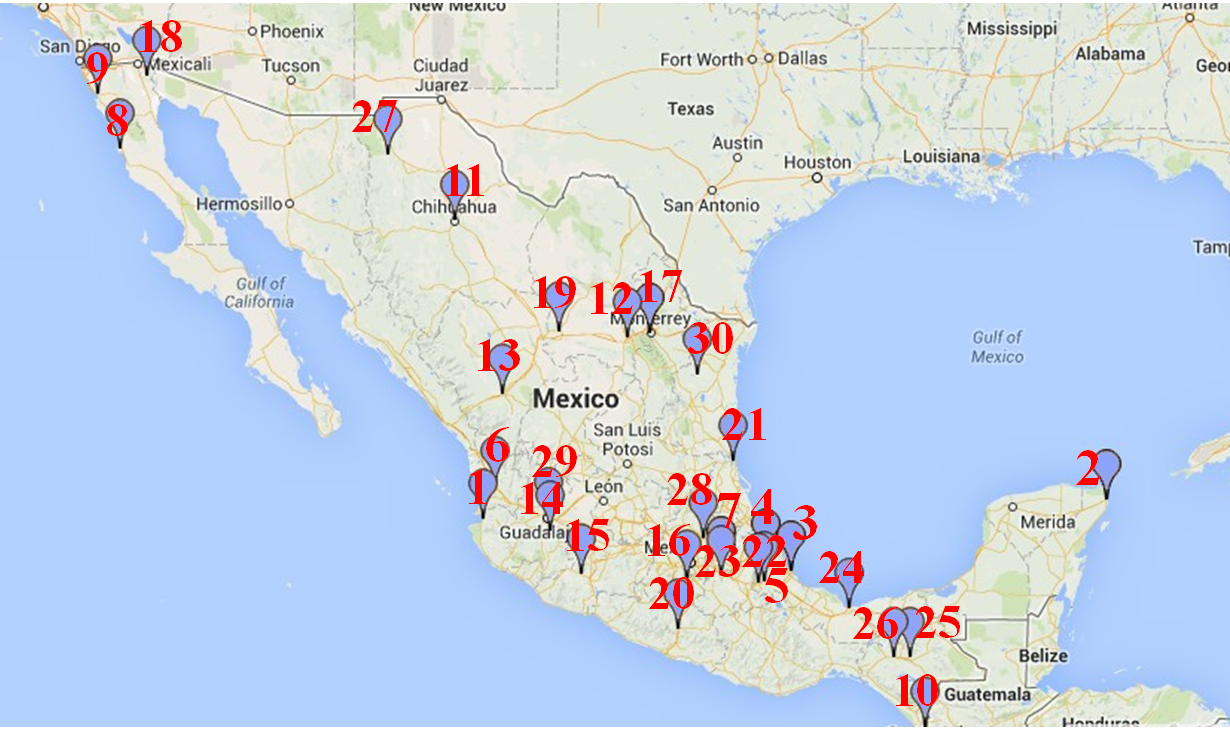
\includegraphics[scale=0.4]{figures/mexico_teacher_protest.png}
\caption{Mexico teacher protest events from Sep 1 to Sep 7, 2013. The blue pins denote protest cities; the numbers in red denote the sequence of
protests as they spread across the country.}
\label{fig:mexico_teacher}
\end{figure}


In this chapter, we focus on Twitter's
user networks during protests
and similar civil unrest activities in Latin America. Our goals
are to model the propagation and growth of contagion-like protest
waves within a social network and to understand the social and
structural dynamics underlying such phenomena. The key problem
is understanding the nature of information propagation among motivated
users of a social network. We have observed that such mass
protests emerge very swiftly and sharply. In Twitterspeak, they
would be considered trending but most such trends quickly decline
on the social network even if not in the physical world. Modeling
protest-related topic propagation on networks involves several challenges.

First, social protest propagation through online media can spread
over large areas more quickly than traditional
methods since users are geographically distributed. For example,
on September 1, 2013, the Mexican government's education reform bill drew
the wrath of teachers country-wide who opposed the reform
(which required regular assessments of their performance as educators).
Twitter was a virtual loudspeaker, providing a platform for organization
and strategization for teachers to put forth their arguments against
the bill. A series of mass teacher protests erupted and spread
from city to city. As shown in Fig.~\ref{fig:mexico_teacher}, we
see the movement spreading over time to different locations with
no obvious visual mobilization pattern. The second challenge is
that Twitter's user network embodies many subgraphs based on
social ties which might afford different propagation rates due to
subgraph-specific structures.

Thus identifying how the cause of a protest is adopted by Twitter users and how mobilization happens in the underlying network is a difficult task.
To address this problem we present an integrated framework with new
theoretical models as well as empirical validation on real Twitter
data for actual protests witnessed in the recent past. Our key
contributions are:

\iffalse
We also focus on the role of community driven information propagation over this bispace. We use \textit{Geometric Brownian Motion} (GBM) and Poisson processes over the mentions network and latent space respectively to model information propagation during mass social movements. When the protest-related information propagation starts, it propagates over the two spaces independently and simultaneously. In the mention network space, the propagation process follows Geometric Brownian diffusion over the defined social network. In the latent space, we believe propagation will obey the Poisson distribution. We introduce a trust function $S_t$ and Brownian distance $d_{ij}$ between users to describe the information propagation mechanism of the mentions network. Suppose that some user $v_i$'s trust with user $v_j$ at time $t$ is $S^{ij}_t$ and the distance from user $v_i$ to user $v_j$ is $d_{ij}$. Only when $ln(S^{ij}_t)$ is no less than the distance $d_{ij}$ is $v_j$ infected by $v_i$.
%We propose that the trust function $S_t$ follows a dynamic geometric Brownian motion
%\begin{equation}\frac{\partial S_t}{S_t} = \mu {dt}+\sigma dW_t
%\end{equation}


In the latent space, we model the propagation as a Poisson distribution, believing that it is difficult to account for all the ways in which information may spread. For a given time interval $T_p$, the probability of infecting users is expressed as $Pr(x=k)=\frac{\lambda^k e^{-\lambda}}{k!}$ where $\lambda$ is the average number of infected users during that time interval $T_p$.
\vspace{2 mm}
\fi

\begin{itemize}
\item
We model the inherent heterogeneity in propagation using a
bispace model, comprised of the Twitter mentions network (where
both globally and locally influential neighbors contribute to a user's
recruitment) and a
latent space (where external exposure to protest-related information is
captured).
\item We focus on the role of community-driven information propagation
over the bispace model. We use geometric Brownian motion (GBM)
over the mentions network and Poisson processes over the latent space to model information propagation during mass social movements.
\item We illustrate the effectiveness of our approach in modeling several key mass protest adoption scenarios in multiple countries of Latin America, viz.
Argentina, Brazil,
Colombia,
Mexico,
Uruguay, and
Venezuela.

\end{itemize}

The rest of this chapter is organized as follows. Section 2 covers related work in the areas of social movements, information diffusion in networks, external influences, and Brownian motion. Section 3 proposes the geometric Brownian motion propagation mechanism. Section 4 introduces the bispace propagation model, especially the model of propagation in latent space. In Section 5, we
present our dataset and experimental setup,
followed by initial experimental findings. Section 6 discusses the
evaluation results for our approach followed by a brief discussion in
Section 7.

\section{Related Work}
We briefly review related work next, which comes from multiple areas.

\par \noindent
{\bf Social movements:}
Oliver and Myers~\cite{oliver1998diffusion}
develop a foundation for theoretical insights of social movements and
describe the limitations of simplified models. The Arab Spring of  2010
served as a context for many
researchers~\cite{gonzalez2011dynamics, bond201261, tufekci2012social, conover2013digital, saad2013mass}
to study the role
social networking sites play in the spread and recruitment
of participants in protests.
A detailed anatomy of
modern social protests is described by Saad-Filho~\cite{saad2013mass}
with the June 2013 anti-government protests in Brazil as a context.
In this work, we study the processes and sociological impacts of protests
in the modern era, fortified by online social networks and the
communities in and around them.\\

\vspace{-0.1in}
\noindent
{\bf Information diffusion in networks:}
Previous studies have approached the modeling of information propagation and
diffusion in social networks through several means, e.g.,
contagion models (SIR~\cite{castellini2007propagation}\, SISa~\cite{hill2010emotions}), diffusion based threshold and cascade models~\cite{kempe2003maximizing}, rise-and-fall patterns~\cite{matsubara2012rise}, coverage models~\cite{singer2012win}, and survival theory~\cite{rodriguez2013modeling}. A good survey of
different models of information diffusion is presented in~\cite{guille2013information}.\\

\vspace{-0.1in}
\noindent
{\bf External influences:}
We believe that the effects of influences that originate external
to the observed diffusion network, such as mass media
and offline spread of information, can impact the way in which information
flows within the online network.
Myers et al.~\cite{myers2012information} study the emergence of URLs
on Twitter with a probabilistic generative process using both
internal and external exposure curves in a contagion-like model.
Similar attention to the role of external factors is
paid by Crane and Sornette~\cite{crane2008robust} for
tracking the popularity of YouTube videos using a diffusion model.
Iwata et al.~\cite{iwata2013discovering} use
a shared cascade Poisson process model to discover
latent influences in social activities such as item adoption.
Using shared parameters among multiple Poisson processes, they were able to simulate sequences of item adoption events. \\

\vspace{-0.1in}
\noindent
{\bf Brownian motion:}
Zhou and colleagues (e.g.,~\cite{zhou2003distance, zhou2003network,
zhou2004network}) develop the notion of Brownian motion on networks
which they
use to discover communities of hierarchical structure both locally
and globally. We extend this approach in this paper
to formulate a propagation algorithm based on geometric Brownian
motion (GBM). Borrowed from statistical physics, GBM has been
used heavily in finance to model stock price movements.
Scale invariance and the ability to model abrupt bumps
along propagation paths are the primary motivations for using GBMs
to model stochastic processes~\cite{tankov2004financial}. \\

\vspace{-0.1in}
\noindent
Our work builds on the concepts
introduced in~\cite{zhou2003network, iwata2013discovering, zhou2003distance, zhou2004network} but differs from the other diffusion models
described earlier by considering both the role of communities of
users and the abrupt nature of propagation of volatile information such as mass social protests. We include the notion of bispace where both latent (attributed to external influences) and observed user network influences are considered. We infer propagation rates for communities in the observed network and allow
implicit recruitment of users into protest actions through a Poisson process.

%!TEX root = ../main.tex
% mainfile: ../main.tex

\section{Formalisms}

\subsection{Basics}
\begin{figure}[th]
\centering
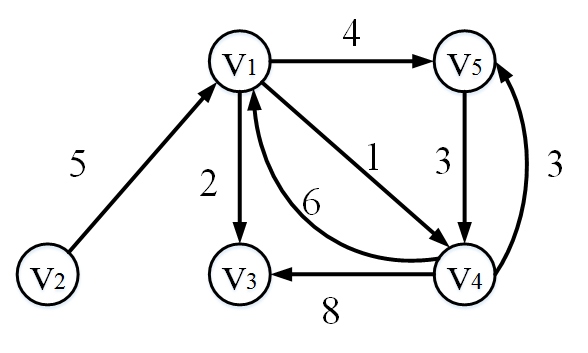
\includegraphics[width=2.4in]{figures/mention_network.png} %?????????????
\caption{An example mentions network. Nodes denote Twitter users,
directed edges denote direction of mentions between users, and edges
are labeled with mention frequency.}
\label{fig:mention_network}
\end{figure}

We model Twitter activity as a network $G(V,E)$ of mentions.
Here, each vertex $v \in V$ represents a Twitter user.
There is a directed edge from user $v_i$ to user $v_j$
if $v_i$ mentions $v_j$ in
a tweet.
We define $\omega_{ij}$ to be the number of tweets in which user $v_i$ mentions user $v_j$. Note that $\omega_{ij}$ is not necessarily equal to $\omega_{ji}$.
Key players such as celebrities and politicians are more
likely to be mentioned by other users, rather than the other way around.
As can be seen in Fig.~\ref{fig:mention_network}, the mentions network
is a directed graph. Weight $w_{14}$ is the number of times Twitter user $v_1$ mentions user $v_4$, which is 1, while $w_{41}$ is 6. Note
that $w_{21}$ is 5, while $w_{12}$ is 0 (not shown).

We define the neighborhood $N(v_i)$ of a user $v_i$ as the set of all users
mentioned by $v_i$, i.e., those for whom there is a directed edge from
$v_i$.
For each user $v_j \in N(v_i)$, we define the Brownian distance from user $v_i$ to $v_j$ to be
\begin{equation}
 d_{ij}=\frac{1}{(\omega_{ij}+1)(\omega_{ji}+1)^\gamma(\eta_{ij}+1)^\gamma}
\end{equation}
Here, $\eta_{ij}$ is the number of common direct neighbors shared by user $v_i$ and user $v_j$~\cite{zhou2004network}. In Fig.~\ref{fig:mention_network}, node $v_1$ and $v_4$ share two common direct neighbors---$v_3$ and $v_5$---and
hence $\eta_{14}$ is 2.

We use the bias coefficient $\gamma \geq 1$ to heuristically
weigh mentions that carry more impact. If $v_i$ mentions $v_j$, meaning that $\omega_{ij} > 0$, we believe this expresses $v_i$'s intention to propagate information to $v_j$.
Since $v_j$ may not know or care about $v_i$ and consequently may seldom or never mention $v_i$, the return mentions, measured by $\omega_{ji}$, are (up)weighted by $\gamma$.
Furthermore, if $v_i$ and $v_j$ share neighbors in the mentions
network, the two users may have a closer relationship than other users
with no shared mentioned Twitter users, and thus this component
is weighted by $\gamma$ as well. A Laplacian-style $(+1)$ correction is used
when there are no counter mentions or no mutual mentions.
Note that for $\gamma = 1$, $d_{ij}$ is an unbiased Brownian distance since $\omega_{ij}$, $\omega_{ji}$, and $\eta_{ij}$ will have the same weight.

\subsection{Trust functions and GBM}
\begin{figure}[ht]
\centering
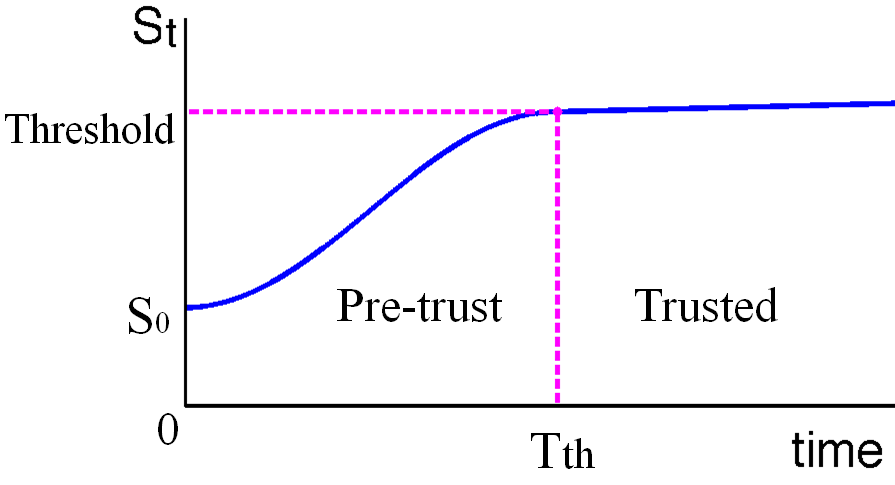
\includegraphics[width=2.4in, height=1.4in]{figures/trustFunction.png} %?????????????
\caption{Trust function. A threshold defines the transition between the
pre-trust and trusted period.}
\label{fig:subgraph}
\end{figure}

Next we introduce the notion of a
trust function $S_t$ which we use to model an individual user's agreement with an idea as expressed in tweets.
(The trust function $S_t$ is a function of the two entities between whom
trust is modeled, but in this section we simplify the notation for
ease of exposition.)
We divide the trust process into a pre-trust
period and a trusted period.
In the pre-trust period, as a user receives new information, that user's trust, $S_t$, increases exponentially until $S_t$ reaches the trust threshold at time $T_{th}$ and enters the trusted period.
In the trusted period, new information increases $S_t$ linearly. For simplicity, an individual user cannot revoke trust once this threshold has been crossed. In our Twitter mentions network, a user's trust in a topic crosses the threshold when they have tweeted about it. During the pre-trust period, we model the
trust function as follows (the coefficient $\mu$ accounts for change in the average value of this stochastic process):
\begin{equation}\frac{d S_t}{S_t} = \mu {dt}\end{equation}
% introduce $\sigma$, $W_t$


We then add a Wiener process $W_t$ to account for stochasticity.
According to the properties of a Wiener process~\cite{oksendal2003stochastic},
$dW_t$ is essentially Gaussian white noise and contributes to our
equation as:
\begin{equation}\frac{d S_t}{S_t} = \mu {dt}+\sigma dW_t\end{equation}
In this way, we modeled the trust function $S_t$ as a geometric Brownian motion (GBM) process which is a continuous-time stochastic process~\cite{oksendal2003stochastic}. Per convention, we call $\mu$ the drift and $\sigma$ the volatility. The drift represents deterministic trends while the volatility refers to the influence of unpredictable events in this model~\cite{wiersema2008brownian}. For simplicity, we consider $\mu$ and $\sigma$ to be constant during the pre-trust period in this chapter. (Our concern here primarily is with this period.)


According to It\={o}'s theorem~\cite{oksendal2003stochastic}, given the initial value $S_0$,
the above stochastic differential equation has the following analytic solution:
\begin{equation}
S_{t}=S_{0}\exp \left(\left(\mu -{\frac  {\sigma ^{2}}{2}}\right)t+\sigma W_{t}\right)
\end{equation}
The above solution for $S_{t}$ is a log-normally distributed random variable with expected value and variance given as~\cite{oksendal2003stochastic}:
\begin{equation}
{  {E}}(S_{t})=S_0e^{{\mu t}}
\end{equation}
\vspace{-1em}
\begin{equation}
 {Var}(S_{t})=S_0^2e^{{2\mu t}}\left(e^{{\sigma ^{2}t}}-1\right)
\end{equation} $S_t$ is a geometric Brownian motion stochastic process, which is typically denoted as $\mathcal{B}(\mu,\sigma)$.
In this chapter we use an initial trust of $S_0 = 1$ without loss of generality.



%\begin{algorithm}
%\label{alg:gbm_prop}
%\SetKwData{Left}{left}\SetKwData{This}{this}\SetKwData{Up}{up}
%\SetKwFunction{Union}{Union}\SetKwFunction{FindCompress}{FindCompress}
%\SetKwInOut{Input}{input}\SetKwInOut{Output}{output}
%\SetAlgoLined
%\Input{mentions network $G(V,E)$, time step $\delta t$, propagation time $T$}
%\Output{infected users}
%        \For{\textrm{each infected user} $v_i \in V$}
%	{	
%	 \For{\textrm{each non-infected user} $v_j \in N(v_i)$}
%	   { set $t_{ij}=0$;}
%	     set $v_i$ as \textrm{not newly infected user}
%        }
% t = 0; \\
%\For{$t \leq T$}{
%    \For{each infected user $v_i \in V$}
%	{  \If{$v_i$ is \textrm{a newly infected user}}
%	   {
%	 \For{\textrm{each non-infected user} $v_j \in N(v_i)$}
%	   { set $t_{ij}=0$;}
%	    set $v_i$ as \textrm{not newly infected user}
%           }	
%	 \For{\textrm{each non-infected user} $v_j \in N(v_i)$} 	
%	   {      set $t_{ij}=t_{ij}+\delta t$ \\
%	   $ln(S_{t}^{ij})\sim \mathcal{N}((\mu - \frac{\sigma^2}{2})t_{ij}, \sigma ^{2}t_{ij})$ \\
%        \If{$ln(S_{t}^{ij})\geq d_{ij} $}
%	   {set \textrm{user $v_j$ as newly infected}}
%        }
%     }
%    $t=t+\delta t;$
%}
%\caption{GBM propagation algorithm}
%\end{algorithm}


\subsection{GBM propagation}
Suppose that user $v_i$ posts a protest-related tweet at time
$t_0$ which indicates that $v_i$ has been recruited or infected.
Whether $v_i$ will infect its neighbor $v_j$ depends on $v_j$'s trust function with $v_i$. For instance, if $v_j$ is a close friend of $v_i$, then it is more likely that $v_j$ will be infected in a short time because of $v_j$'s trust in $v_i$. But if $v_j$ is not a very close friend of $v_i$, then it might take a long time to build $v_j$'s trust with $v_i$ and to accept $v_i$'s status. Only after $v_j$'s trust with $v_i$ crosses some threshold, $v_j$ gets infected.

For better quantitative analysis, we consider $d_{ij}$ to be the trust threshold. After crossing this threshold, $v_j$ will agree with $v_i$'s opinion. According to the properties of GBMs, the trust function $S_t$ grows continuously over time. This implies that, if some user is infected, all of that user's neighbors will eventually get infected given enough time for diffusion.

Since we assume a user cannot revoke trust, his or her status will never change once infected. Based on the above assumptions, we now detail our process for GBM propagation through the mentions network; see Algorithm 1. Since GBM is a time-continuous stochastic process, we discretize
time using time steps of duration $\delta t$ each.
At the start of the simulation, all infected users are considered as newly infected users.
Assume that
the complete mass protest propagation duration is $T$. Once a user $v_i$ becomes infected, the node is marked as a newly infected user, and the
new status begins to affect the statuses of the neighbors, i.e., $N(v_i)$. For each user $v_j \in N(v_i)$, we use $t_{ij}=0$ to initialize the time
instant from which $v_i$ begins to affect $v_j$.
After all the time variables $t_{ij}$ of $N(v_i)$
are so initialized,
user $v_i$'s status is updated to reflect that $v_i$ is no longer
a newly infected user,
to avoid duplicate initializations.


Suppose that at current time $t$, $v_j$'s trust with $v_i$ is denoted as $S_{t}^{ij}$. According to the GBM properties, $ln(S_{t}^{ij})$ is a Gaussian variable given by:
\vspace{-0.5em}
\begin{equation}
ln(S_{t}^{ij})\sim \mathcal{N}((\mu - \frac{\sigma^2}{2})t, \sigma ^{2}t)
\end{equation}

If at time $t$, $ln(S_{t}^{ij})\geq d_{ij}$, this means that $v_j$ gets infected since $v_j$'s trust with $v_i$ is bigger than the distance $d_{ij}$. Now $v_j$ begins to affect his or her own neighbors. Instead at
time $t$, if $ln(S_{t}^{ij})< d_{ij}$, then at the next time step, $t+\delta t$, the  trust is still a Gaussian variable, but with higher expectation and variance: \begin{equation}
ln(S_{t+\delta t}^{ij})\sim \mathcal{N}((\mu - \frac{\sigma^2}{2})(t+\delta t), \sigma ^{2}(t+\delta t))
\end{equation}




\subsection{GBM parameter estimation}
We use past protest events in
which Twitter played a significant role in propagation to train
our GBM model parameters. For each user who gets
infected we record their Brownian distance and infection time. Suppose $v_j$ gets infected by $v_i$ after time $t_{ij}$; then as per our propagation model, we claim that $v_j$'s trust function $S_t^{ij}$ with $v_i$ holds:
\begin{equation}
ln(S_t^{ij}) \geq d_{ij}
\end{equation}
where $d_{ij}$ is the Brownian distance from $v_i$ to $v_j$. For the convenience of parameter estimation, we can assume that $ln(S_t^{ij}) = d_{ij}$. It
then follows that $d_{ij}$ is a normally distributed random variable which can be expressed as:
\begin{equation}
d_{ij}\sim \mathcal{N}((\mu - \frac{\sigma^2}{2})t_{ij}, \sigma ^{2}t_{ij})
\end{equation}
Because during the parameter estimation process, for each infected user $v_j$, we are not interested in exactly which
user gets $v_j$ infected, we use $x_j = d_{ij}$, and $\tau_j = t_{ij}$ in the following part of this section for simplicity. The set of $n$ users that are infected during the infection process have independent infection rates, and we get the following likelihood function:

\begin{equation*}
{\mathcal  {L}}(\theta, \sigma^2 \,|\,v_{1},\ldots ,v_{n})=\prod _{{j=1}}^{n}\frac{1}{\sigma\sqrt{2\pi \tau_j}}exp(-\frac{(x_j-(\mu-\frac{\sigma^2}{2})\tau_j)^2}{2\sigma^2\tau_j})
\end{equation*}

The optimal estimators can be obtained by maximizing the above likelihood function.
We differentiate the natural logarithm of the likelihood function above in terms of $\mu$ and $\sigma$, and set them to zeros. By solving the
two equations simultaneously, we obtain the optimal estimators $\hat{\mu}$ and $\hat{\sigma^2}$.

%By maximum posteriori probability criterion, we get
%
%\begin{equation}
%\hat{\mathcal  \sigma^2} =\frac{{\sum_{j=1}^{n}\frac{(x_j-k)^2}{\tau_j}}} {{\sum_{j=1}^{n}(x_j-k)+n}}
%\end{equation}
%
%\begin{equation}
%\hat{\mathcal  \mu} =\frac{{\sum_{j=1}^{n}x_j}+ \frac{\hat{\sigma^2}}{2}{\sum_{j=1}^{n}\tau_j}}   {{\sum_{j=1}^{n}\tau_j}}
%\end{equation}
%where, \begin{equation}
%k=\frac{{\sum_{j=1}^{n}x_j}}{{\sum_{j=1}^{n}\tau_j}}
%\end{equation}
%The parameter estimation process has linear complexity.

%!TEX root = ../main.tex
% mainfile: ../main.tex

\begin{figure}[Ht]
\centering
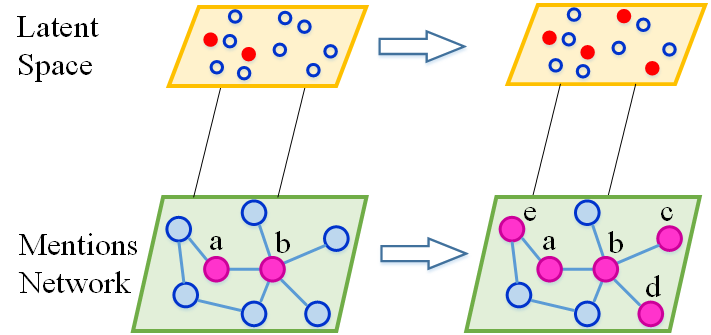
\includegraphics[width=3in] {figures/Bio-space.png}
\caption{Bispace propagation model. In the latent space, users infections
are explained by a Poisson model, and the red nodes denote the infected users
from one time step to another.
In the mentions network space, users are infected according to the
GBM model. Here, the purple nodes (a, b, c, d, e) denote
user infections explained by the GBM model. }
\label{fig:bi-space}
\end{figure}

\section{Bispace Propagation Model}
Many information diffusion models assume that propagation occurs over a single domain.
However, it is hard to build a complete, exhaustive network of interactions.
For instance, consider building a network based only on which Twitter users follow which other users. This network will miss interactions such as retweets and mentions and the effect of influences originating
outside of Twitter. Therefore, considering only a single space will make it difficult to account for all possible factors that influence the spread of information.
In this study, we propose a bispace diffusion model that accounts for two domains of diffusion: the observed social network and the latent space, as can be seen in Fig.~\ref{fig:bi-space}.
In our case, the observed user space is the Twitter mentions network,
whereas the latent space refers to any interactions outside of this network.
To account for varying diffusion dynamics, each space is intended to have
its own propagation model.
As described earlier, we model propagation through the Twitters mentions network as Geometric Brownian motion. We use the Poisson distribution to describe information propagation in the latent space.

\subsection{GBM with Communities}
\begin{figure}[t]
\centering
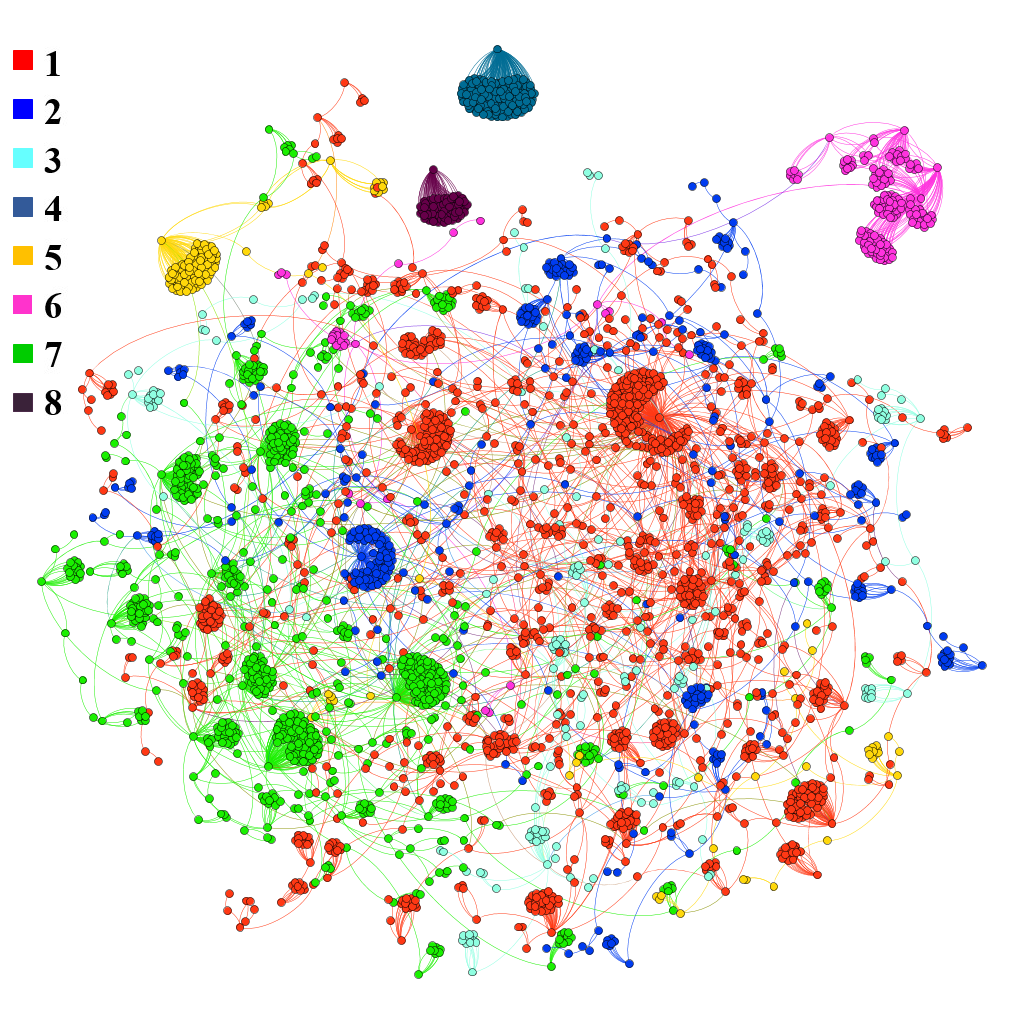
\includegraphics[width=3.3in] {figures/4_teacher_major_community.png}
\caption{Major communities of teacher protest events (Sep 1 to Sep 12, 2013,
Mexico).}
\label{fig:teacher_major_community}
\end{figure}


\begin{figure}[t]
\centering
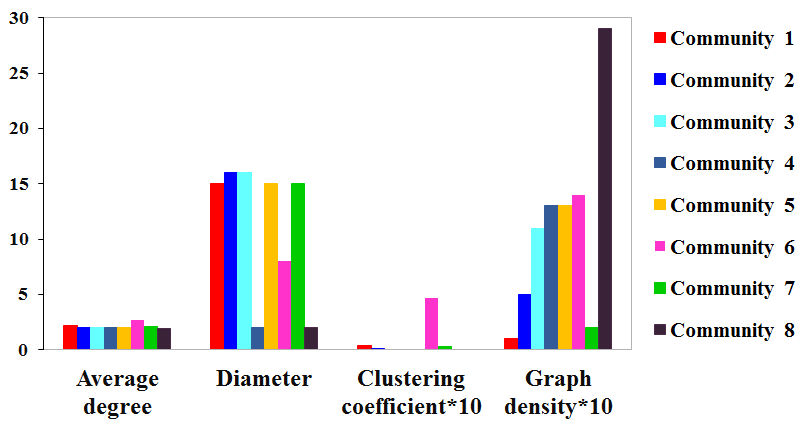
\includegraphics[width=4in, height=2in] {figures/4teacher-community-parameters.png}
\vspace{-4mm}
\caption{Key graph properties of communities underlying the Mexican teacher protest events.}
\label{fig:teacher_community_parameters0}
\vspace{-4mm}
\end{figure}

Within networks, a community refers to the appearance of densely connected groups of vertices, with sparse connections between each group~\cite{newman2006modularity}.
Instead of treating the whole network as a single propagation space,
we use network structure to further split the network into communities.
For our mentions network we use the Louvain method~\cite{blondel2008fast} for community detection to split the network into groups of users. For each community of users we can calculate classical graph features such as average degree, diameter, density, and clustering coefficient with which we can characterize them. In Fig.~\ref{fig:teacher_community_parameters0} we plot several features for each of the 8 communities found in the case study of Mexican teachers protest of 2013. Diameter $r = \max dist(v_i, v_j)$ is the length (in number of edges) of the longest geodesic path between any nodes $v_i$ and $v_j$~\cite{newman2003structure}. The clustering coefficient $c_i$ is the proportion of node $v_i$'s neighbors that are connected. Graph density is defined as $\frac{2|E|}{|V|(|V|-1)}$ where $E$ is the number of edges and $V$ is the
number of nodes~\cite{scott2011sage}. As shown in Fig.~\ref{fig:teacher_community_parameters0}, diameter and graph density vary considerably.


\begin{figure}[t]
\centering
\subfigure[Raw data]{
   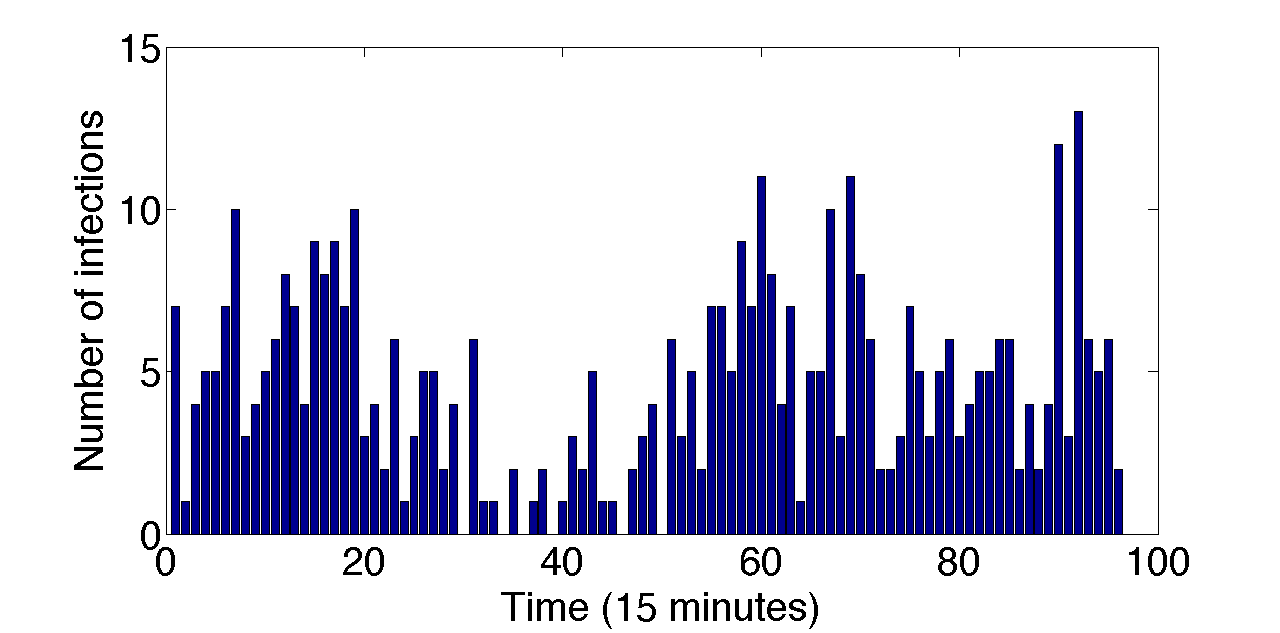
\includegraphics[width=3in,height=1.5in] {figures/Poisson_realData.png}
  \label{fig:Poisson_Sep3}
 }
 \subfigure[Poisson distribution model]{
   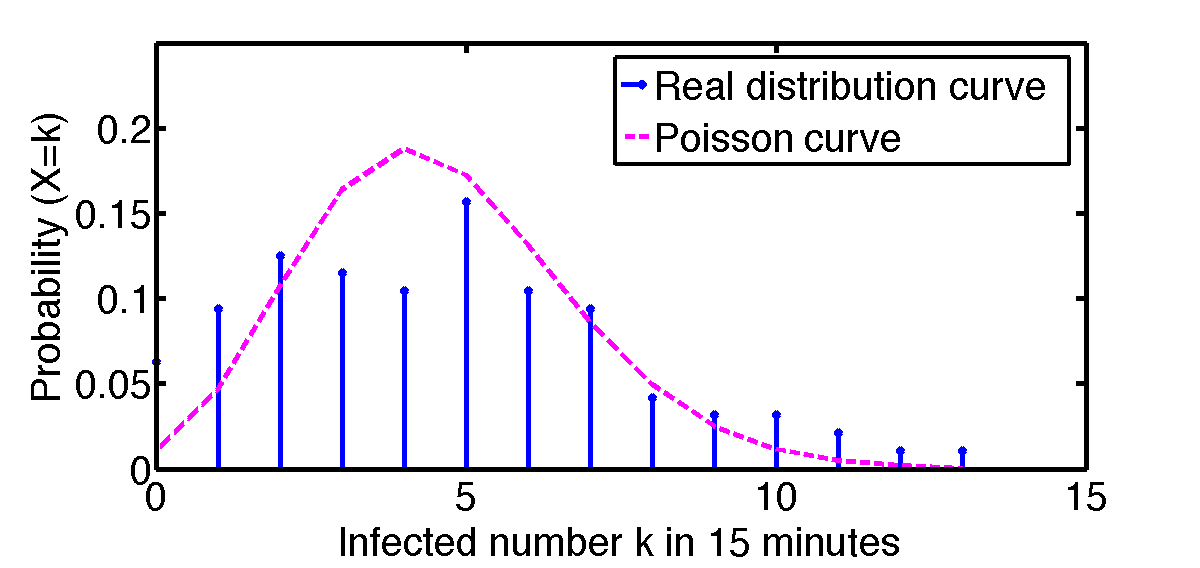
\includegraphics[width=3in,height=1.5in] {figures/poissonianCurve.png}
  \label{fig:poissonianCurve}
 }
\caption{Poisson distribution in latent space propagation. (a) shows the raw data outside of the mentions network of teacher protest events on Sep 3, 2013. (b) shows the probability distribution of the number of
infections.}
\label{fig:Poisson}
\end{figure}






\begin{table*}[t]
\label{table:massprotests}
\caption{Mass protests studied in this chapter.}
\centering
\tiny
%\begin{tabular}{p{0.05\linewidth}p{0.25\linewidth}p{0.20\linewidth}p{0.05\linewidth}p{0.05\linewidth}p{0.05\linewidth}}
\begin{tabular}{lp{0.25\textwidth}p{0.25\linewidth}lll}
\hline \\
No. & Event & Hashtags & Country & Affected cities & Event date(s) \\
\hline \\
1. & YoSoy132 student movement & \#LaMarchaYoSoy132, \#YoSoy132, \#132, \#soy132 & Mexico & Nationwide & 2012-05-17 to 2012-05-25 \\ \\
2. & Anti-government protests against tax reform and other policies pursued by President Juan Manuel Santos & \#CacerolazoPaSantos, \#5D & Colombia & Nationwide & 2012-12-05 \\ \\
3. & Education reform protests by teachers& \#ReformaEducativa & Mexico & Nationwide & 2013-09-01  \\ \\
4. & Social protests against violence and crime  &	\#UruguayosIndignados, \mbox{\#HartosDeLaViolencia} & Uruguay & Montevideo & 2012-05-14 \\ \\
5. & Protests against the ``media law'' & \#LorenzettiNoMeFalles, \#MediosBuitres & Argentina & Buenos Aires & 2012-11-27 \\ \\
6. & Protests against Senate President Renan Calheiros's election & \#STFjulgueRenan, \mbox{\#SocorroJoaquim}, \#ForaRenan & Brazil & Nationwide& 2013-02-22 to 2013-02-26 \\ \\
7. & Anti-government student protests against abuse of public media for election campaign  & \#ConatelCareTabla & Venezuela & Caracas & 2013-03-20 \\[1ex]
\hline
\end{tabular}
\end{table*}




With the observed network further split into several communities, each community is intended to have its own model parameters for GBM. In GBM, $ln(S_t^{ij})$
is a Gaussian distribution $\mathcal{N}((\mu - \frac{\sigma^2}{2})t, \sigma ^{2}t)$. We assume that each user within a community shares the same $\mu$ and $\sigma$ so that each community has its characteristic $\mu$ and $\sigma$. As information propagates through the mentions network, it may pass through different communities.
For an infected user $v_i$ and one of the non-infected
neighbors $v_j \in N(v_i)$, we assume the following propagation
strategy:
\begin{itemize}
    \item If $v_i$ and $v_j$ are in the same community $c_i$, the propagation process will follow $\mathcal{B}_{c_i}(\mu_{c_i}, \sigma_{c_i}^2)$.
        %In this case, we consider the rest of the mention network as part of that user's community, ${c_i}$.
    \item Propagation from one community to another happens as per the source community's model parameters. For instance, for propagation from community ${c_i}$ to community ${c_j}$, we will use the source community ${c_i}$'s GBM parameters.
    \item After information propagates into a different community, it will spread according to the new community's parameters. Once the information has entered community ${c_j}$ from community ${c_i}$, subsequent infections henceforth
will use community ${c_j}$'s parameters.
\end{itemize}

\noindent
At each time step we use the $\mu$ and $\sigma$ of any given node's current community for propagation from that node.
\subsection{Propagation in Latent Space}
As mentioned before, in the latent space, we are modeling unobserved interactions of users. Since there are so many factors that might affect the dissemination of information, such as news outlets, word-of-mouth, it is reasonable to assume that the probability of the number of newly infected users in a given time interval satisfies the Poisson distribution~\cite{haight1967handbook} in the latent space.

For each node in the mentions network, it can only be infected by the GBM process. However, for those isolated users outside the mentions network, it is only possible that they get infected via the mechanics of the Poisson process.
(Recall that in the GBM process, users get infected primarily
via their neighbors.) We use $X$ to represent the number of infected users
with time interval $\delta t$ and so the probability of the infected users is
given by:
\begin{equation}\Pr(X=k)= \frac{\lambda^k e^{-\lambda}}{k!}\end{equation}
To obtain an estimator of $\lambda$, we can only use information
about Twitter users who are outside the mentions network as our training dataset. We count the infected users outside the mentions network with time interval of 15 minutes during the Mexican teachers protest, and plot them as shown in Fig.~\ref{fig:Poisson_Sep3}.
Adequately modelable by a Poisson distribution, we use the average value as the estimate of $\lambda$. Fig.~\ref{fig:poissonianCurve} depicts the Poisson distribution fit with $\hat{\lambda}=4.18$. If there are $M_0$ isolated users, the probability of each of these users to get infected in time interval $\delta t$ is $\lambda/M_0$.
To summarize, for any user not in the mentions network, infection
is only possible via the Poisson process. For a user who is already in the
mentions network, infection can only happen via the GBM process over the mentions network, as described earlier.

%!TEX root = ../main.tex
% mainfile: ../main.tex

\section{Experiments}
\subsection{Dataset description}

The study described in this paper uses two datasets: (i)
a gold standard report (GSR) of social unrest events in Latin America
provided by MITRE that we use to define
major mass protest events, and (ii)
tweets collected over 14 months from May 2012 to September 2013 from 20
Latin American countries.

The GSR documents each civil unrest event by location, date, type
of protest, and specifies the national news articles that
first reported the event. For protests that were prominent on Twitter, the
GSR news articles often report hashtags which were used by protestors
on social media. We selected only those GSR events for which we
were able to find such hashtags. This process resulted in 64
unique hashtags related to 40 different protest that occurred
in Latin America since May 2012. In Table 1 we list a few of
these events from our study.

Our Twitter dataset was built by querying Datasift's streaming API. Each tweet payload includes crucial metadata along with the tweet's content. Though tweets from GPS-enabled devices include geographic coordinates, the percentage of such tweets in the collected sample was too low to be useful.

For this study, we further filtered tweets by removing those that do not contain hashtags relevant to a specific protest. Since most tweets do not have location data, we estimate their location by geocoding the tweet based on each tweet's content and properties of its user. We developed our own geocoding library that uses the World Gazetteer (http://archive.is/srm8P) database to lookup location names and geographic coordinates. Tweets can be geocoded to the user's location at the time of tweeting or a location of interest about which the user is tweeting. We focused on event geolocation, which looks for location or landmark names, such as \textit{Plaza de la Independencia} or \textit{Quito, Ecuador}, in a tweet's text.  We generated a list of 2000 landmarks by extracting place names mentioned in GSR events which had high mutual information to civil unrest. In cases where no event location was found in a tweet's text, we use geo-coordinates or self-reported location string in the tweet's metadata.

Using the above pipeline we were able to extract and geolocate $20,227,830$ unique users to build our mentions network from the filtered tweets that were spread over daily sub-networks.


\begin{figure}[t]
\centering
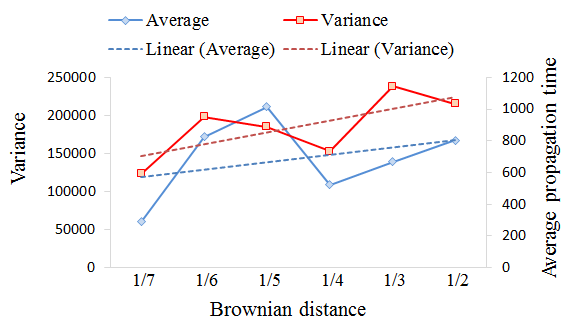
\includegraphics[width=3.2in] {figures/infectdTime.png}
\caption{Brownian distance vs propagation time
for teacher protest events.}
\label{fig:timecurve}
\end{figure}




\begin{figure}[t]
\centering
\subfigure[Simulation without community]{
   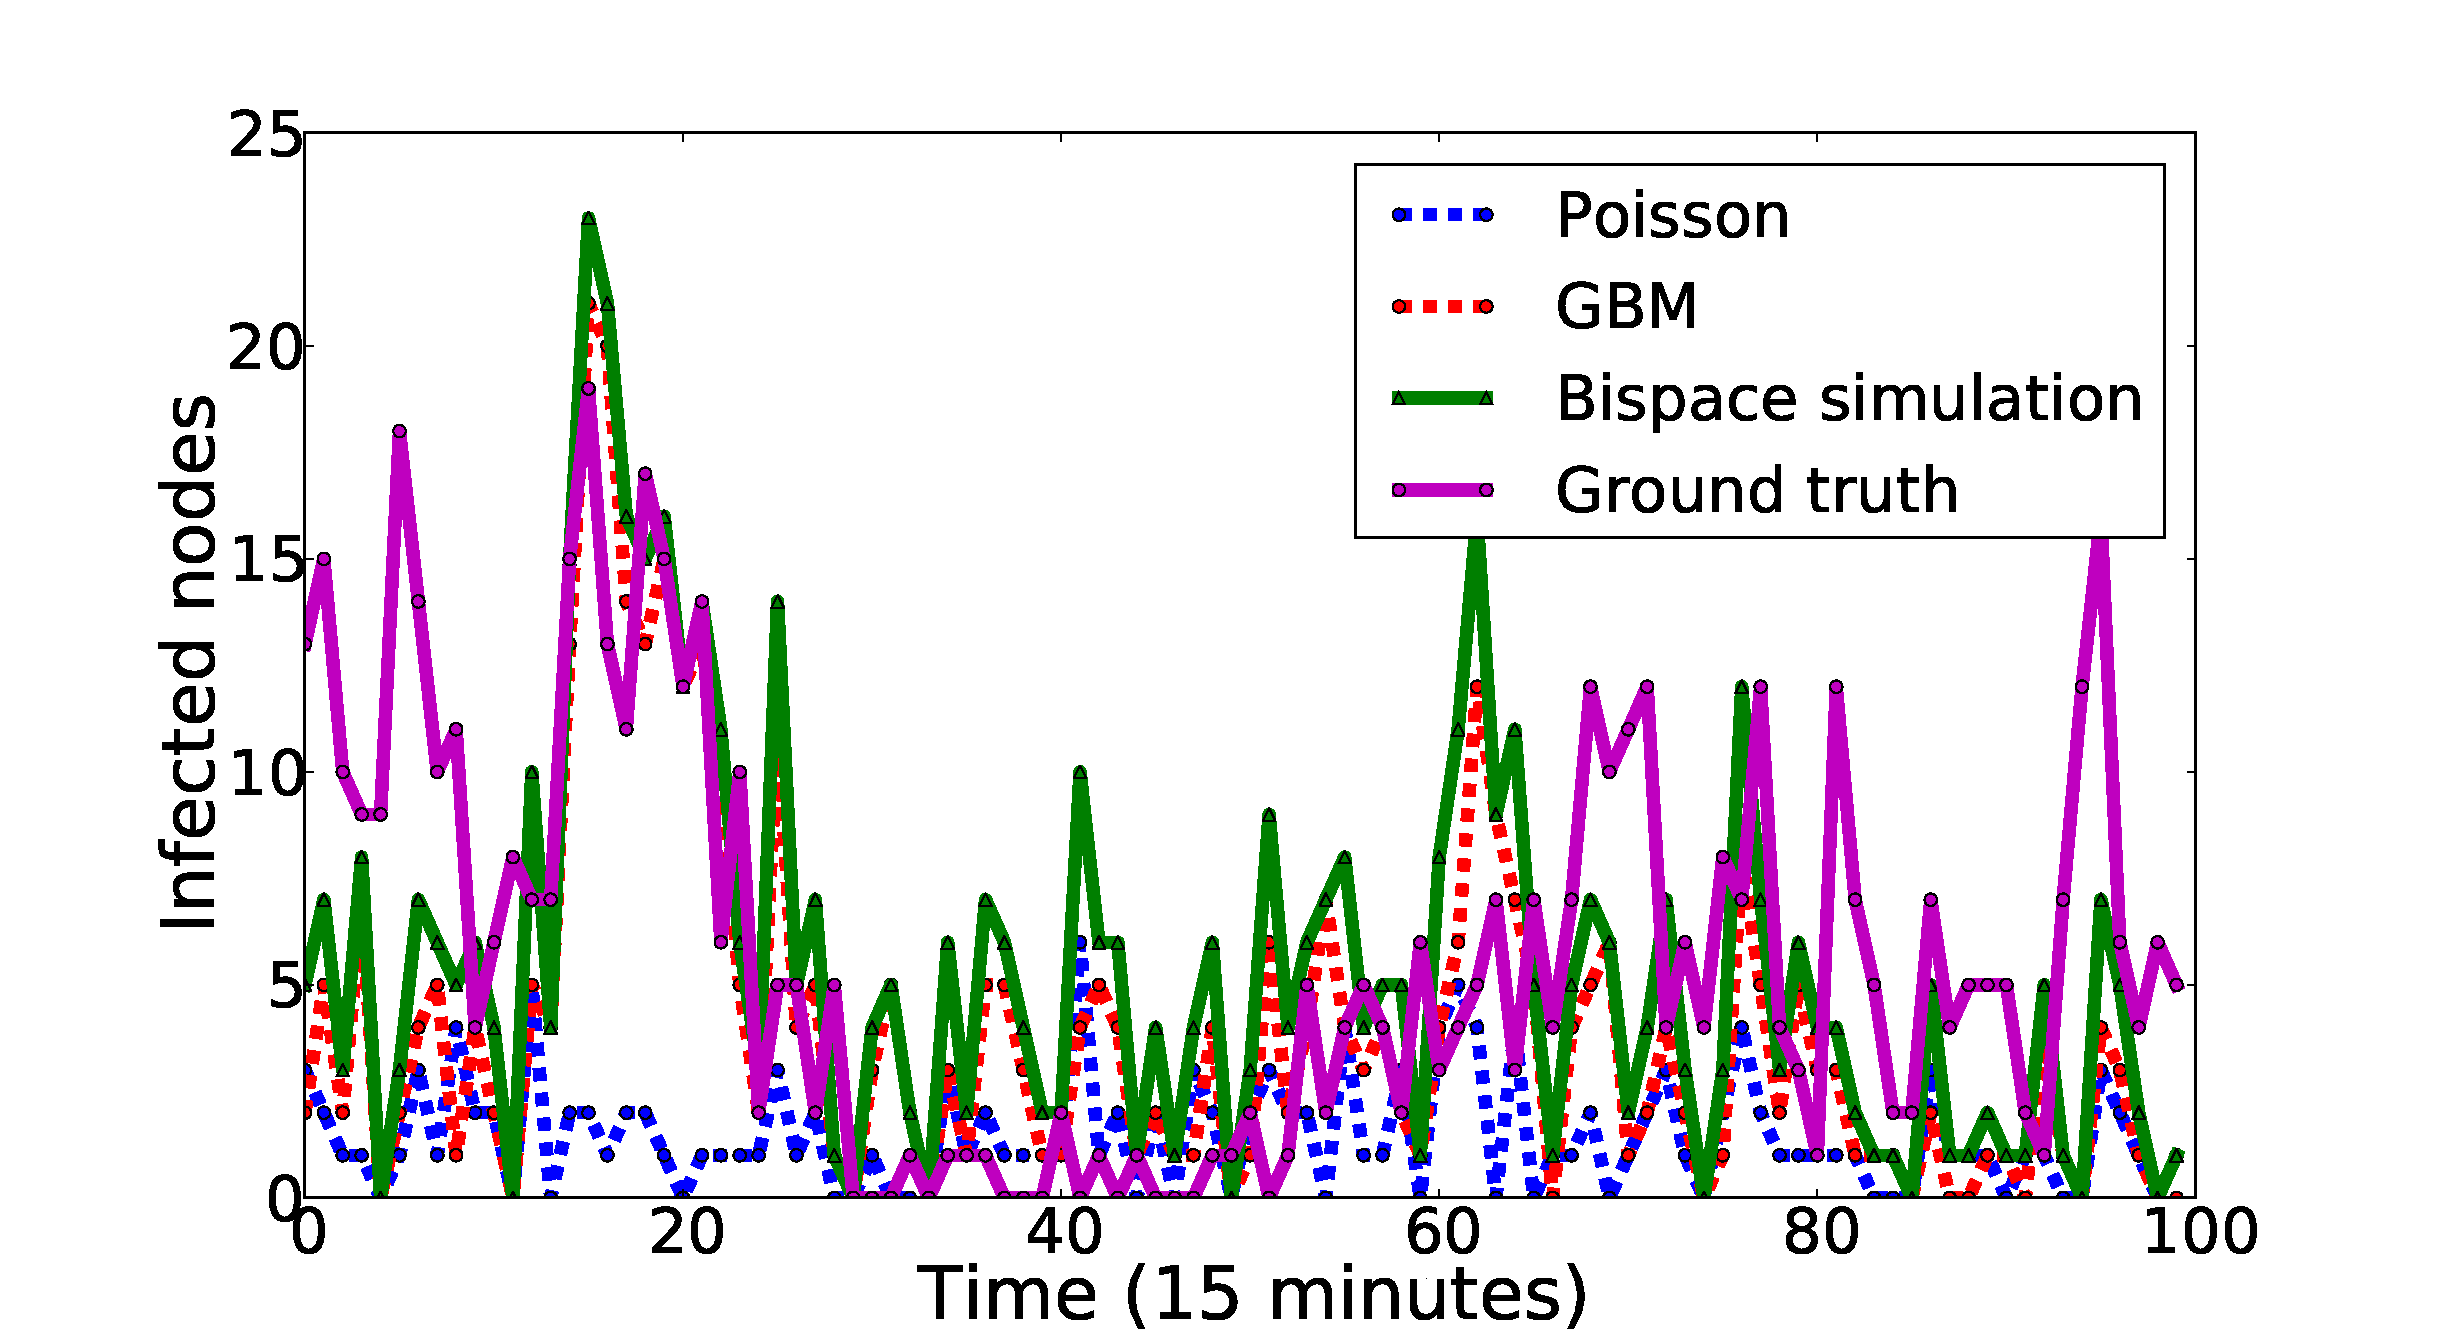
\includegraphics[width=3in,height=1.6in] {figures/1-yosoy-without-community-final.pdf}
  \label{fig:yosou_no_community}
 }
 \subfigure[Simulation with community]{
   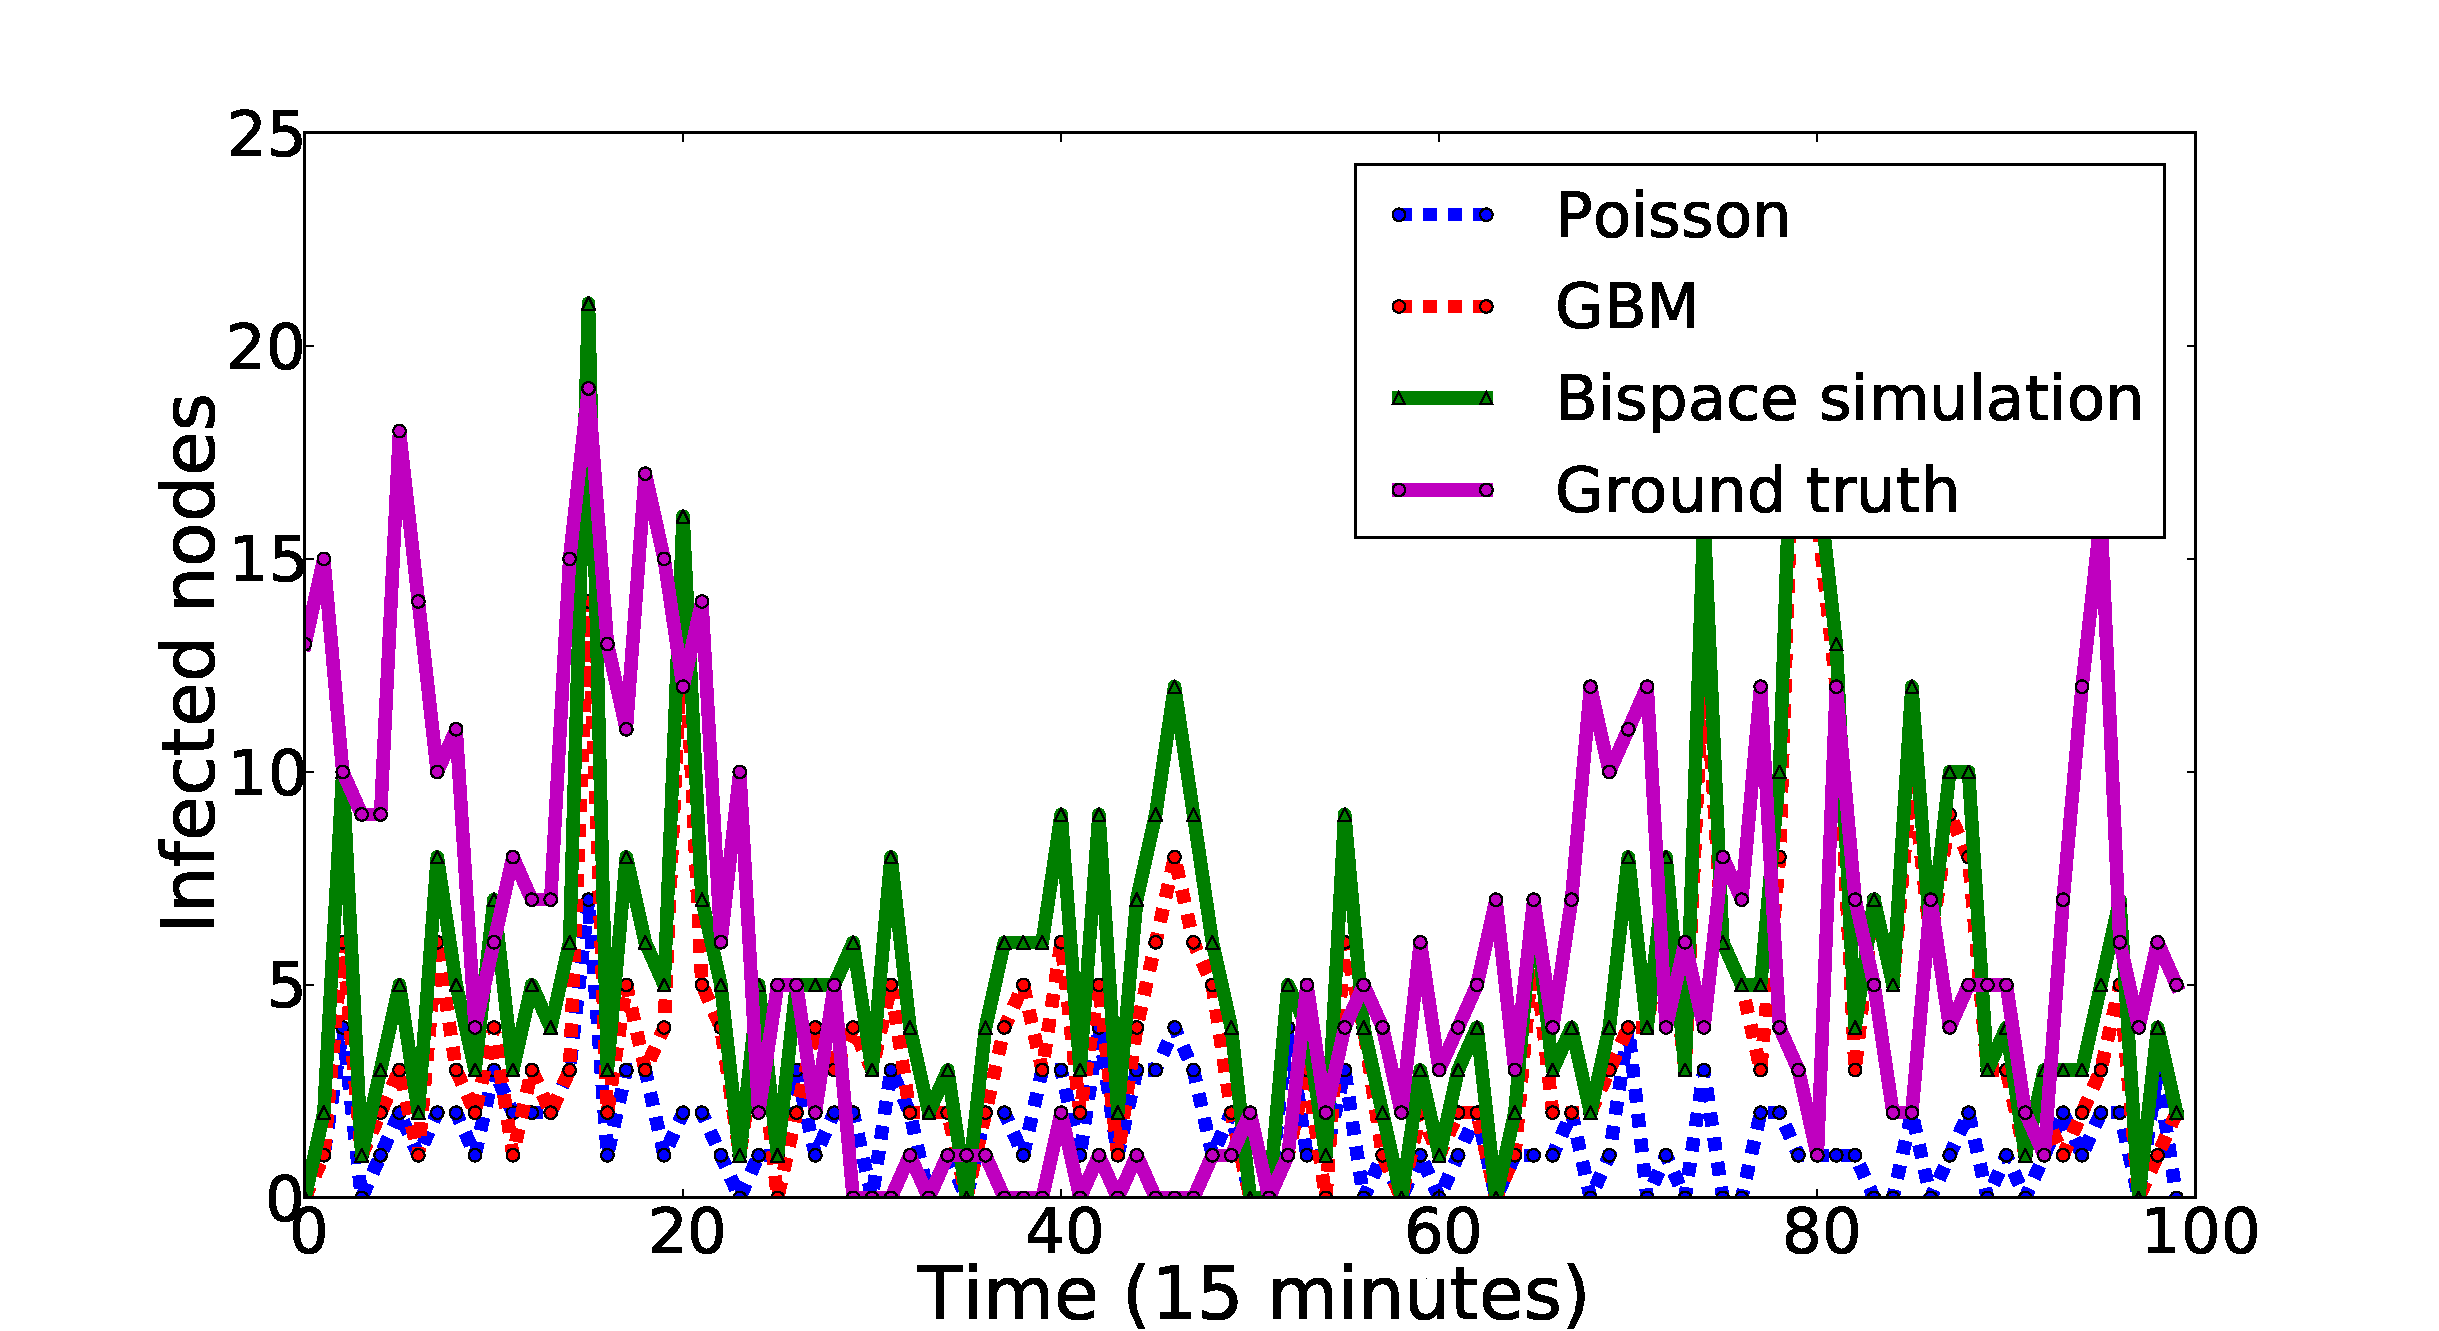
\includegraphics[width=3in,height=1.6in] {figures/1-yosoy-with-community-final.pdf}
  \label{fig:yosou_community}
 }
\caption{GBM and Poisson propagation simulation for Yosoy protests
(Mexico) on May 19, 2012.}
\label{fig:1Yosoy2012may}
\end{figure}


\begin{figure}[th]
\centering
\subfigure[Simulation without community]{
   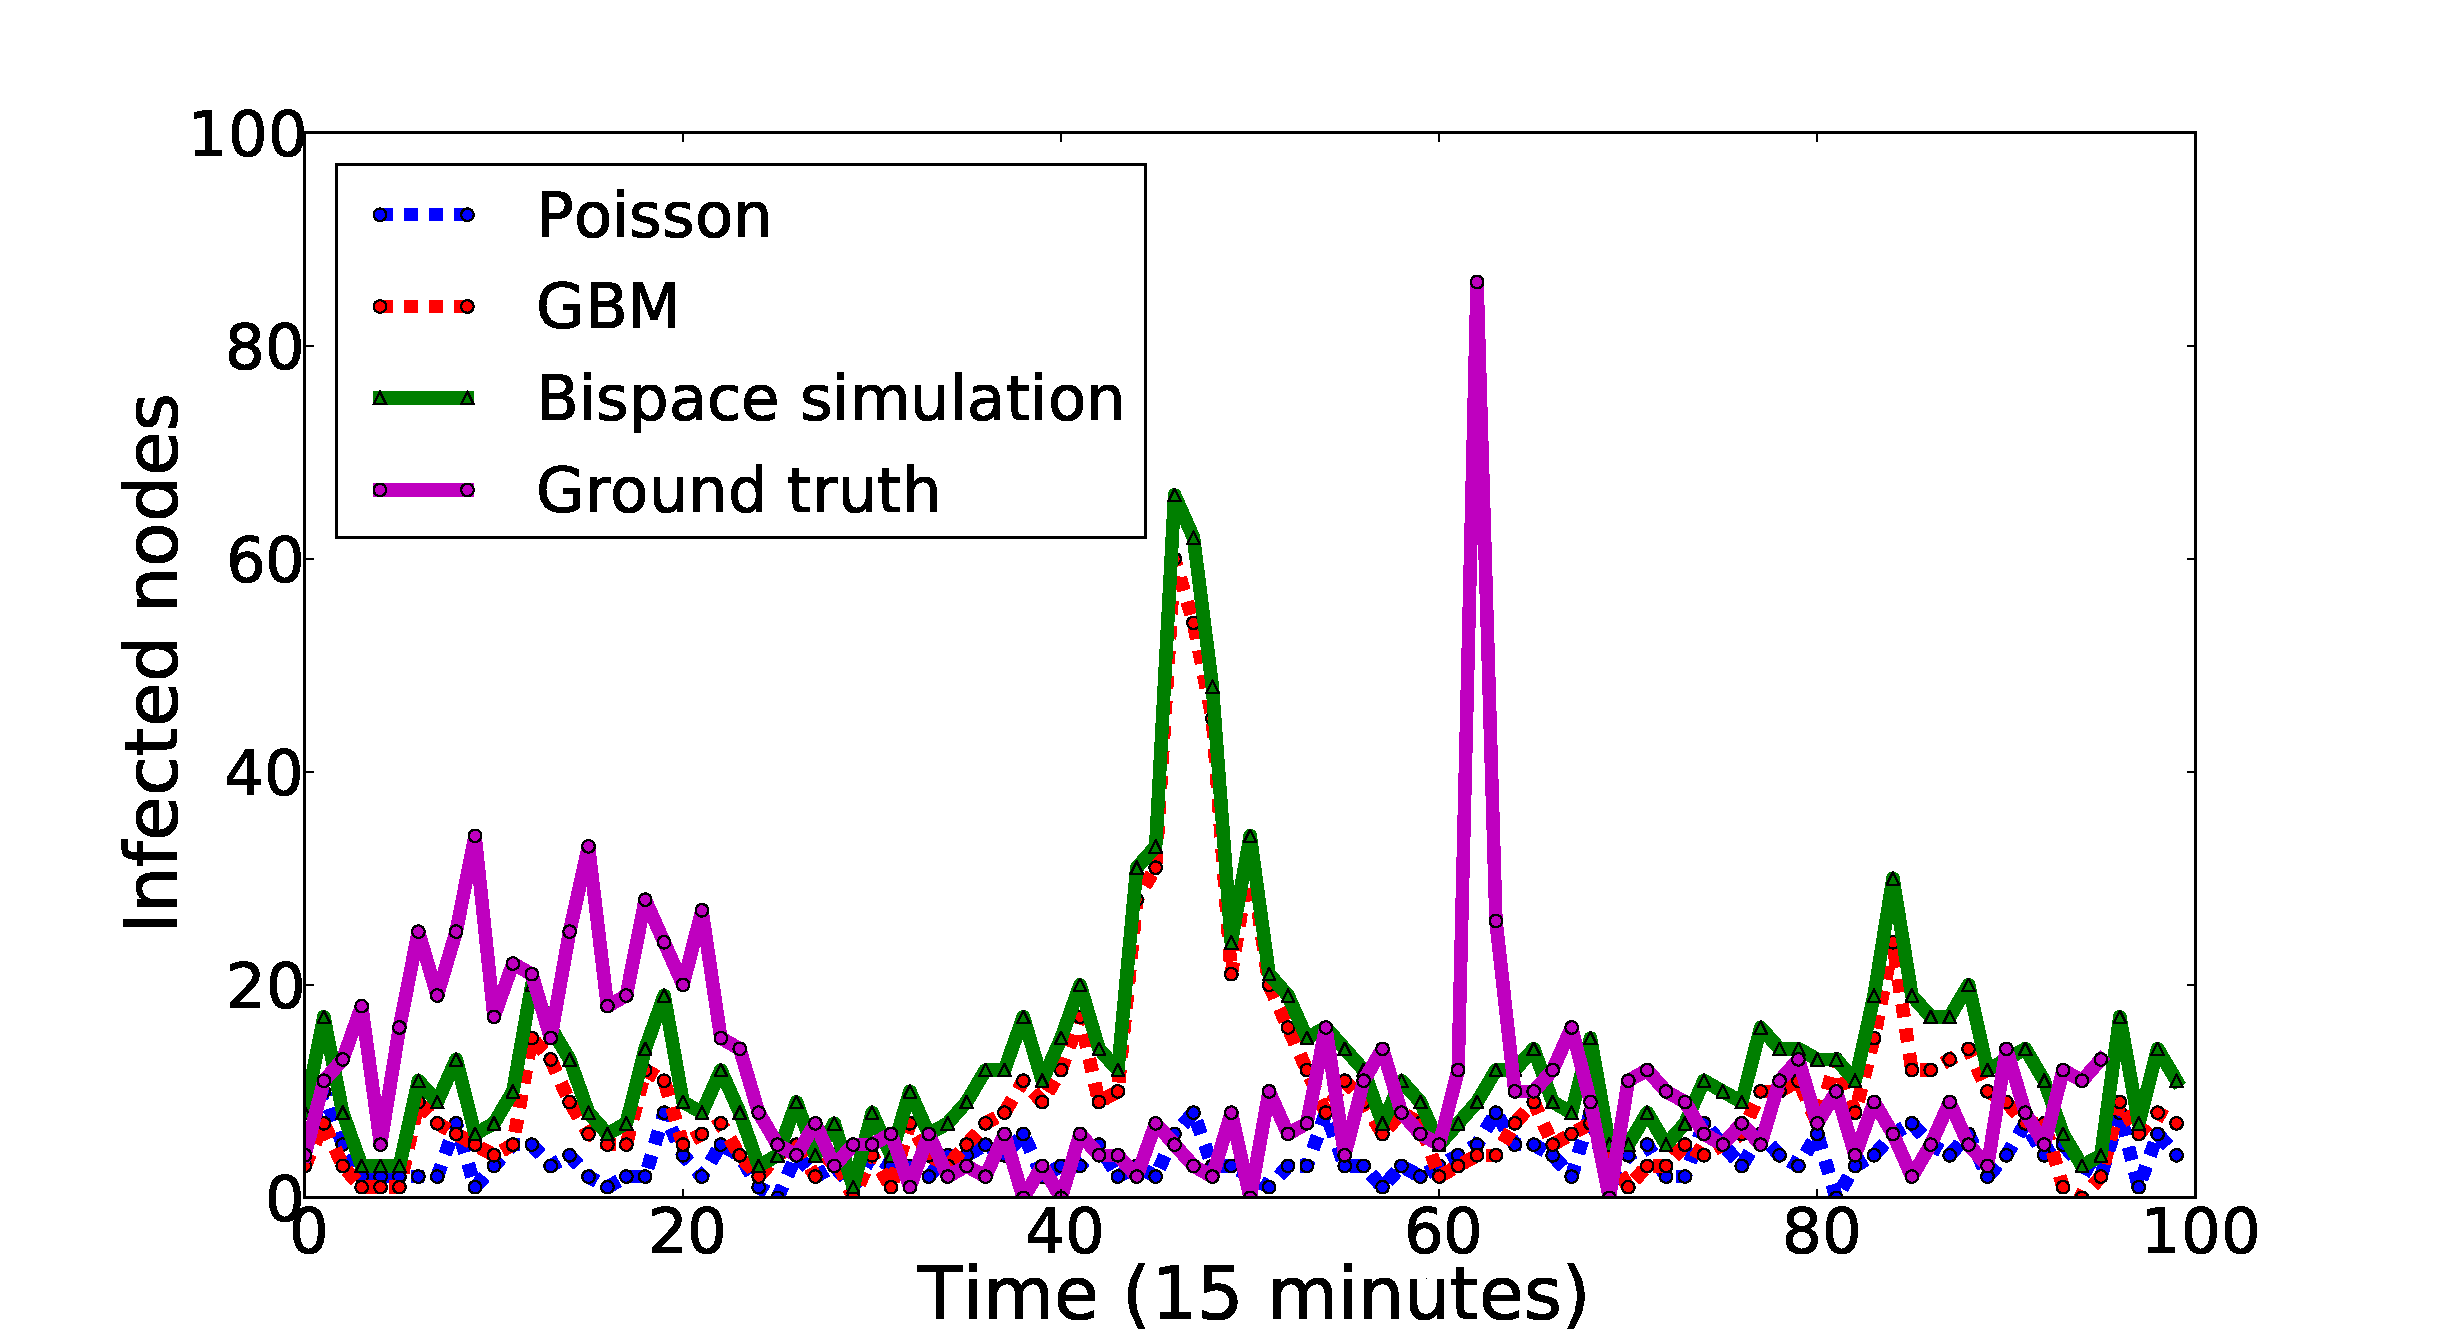
\includegraphics[width=3in,height=1.6in] {figures/4-teacher-without-community-final.pdf}
  \label{fig:teacher_no_community}
 }
 \subfigure[Simulation with community]{
   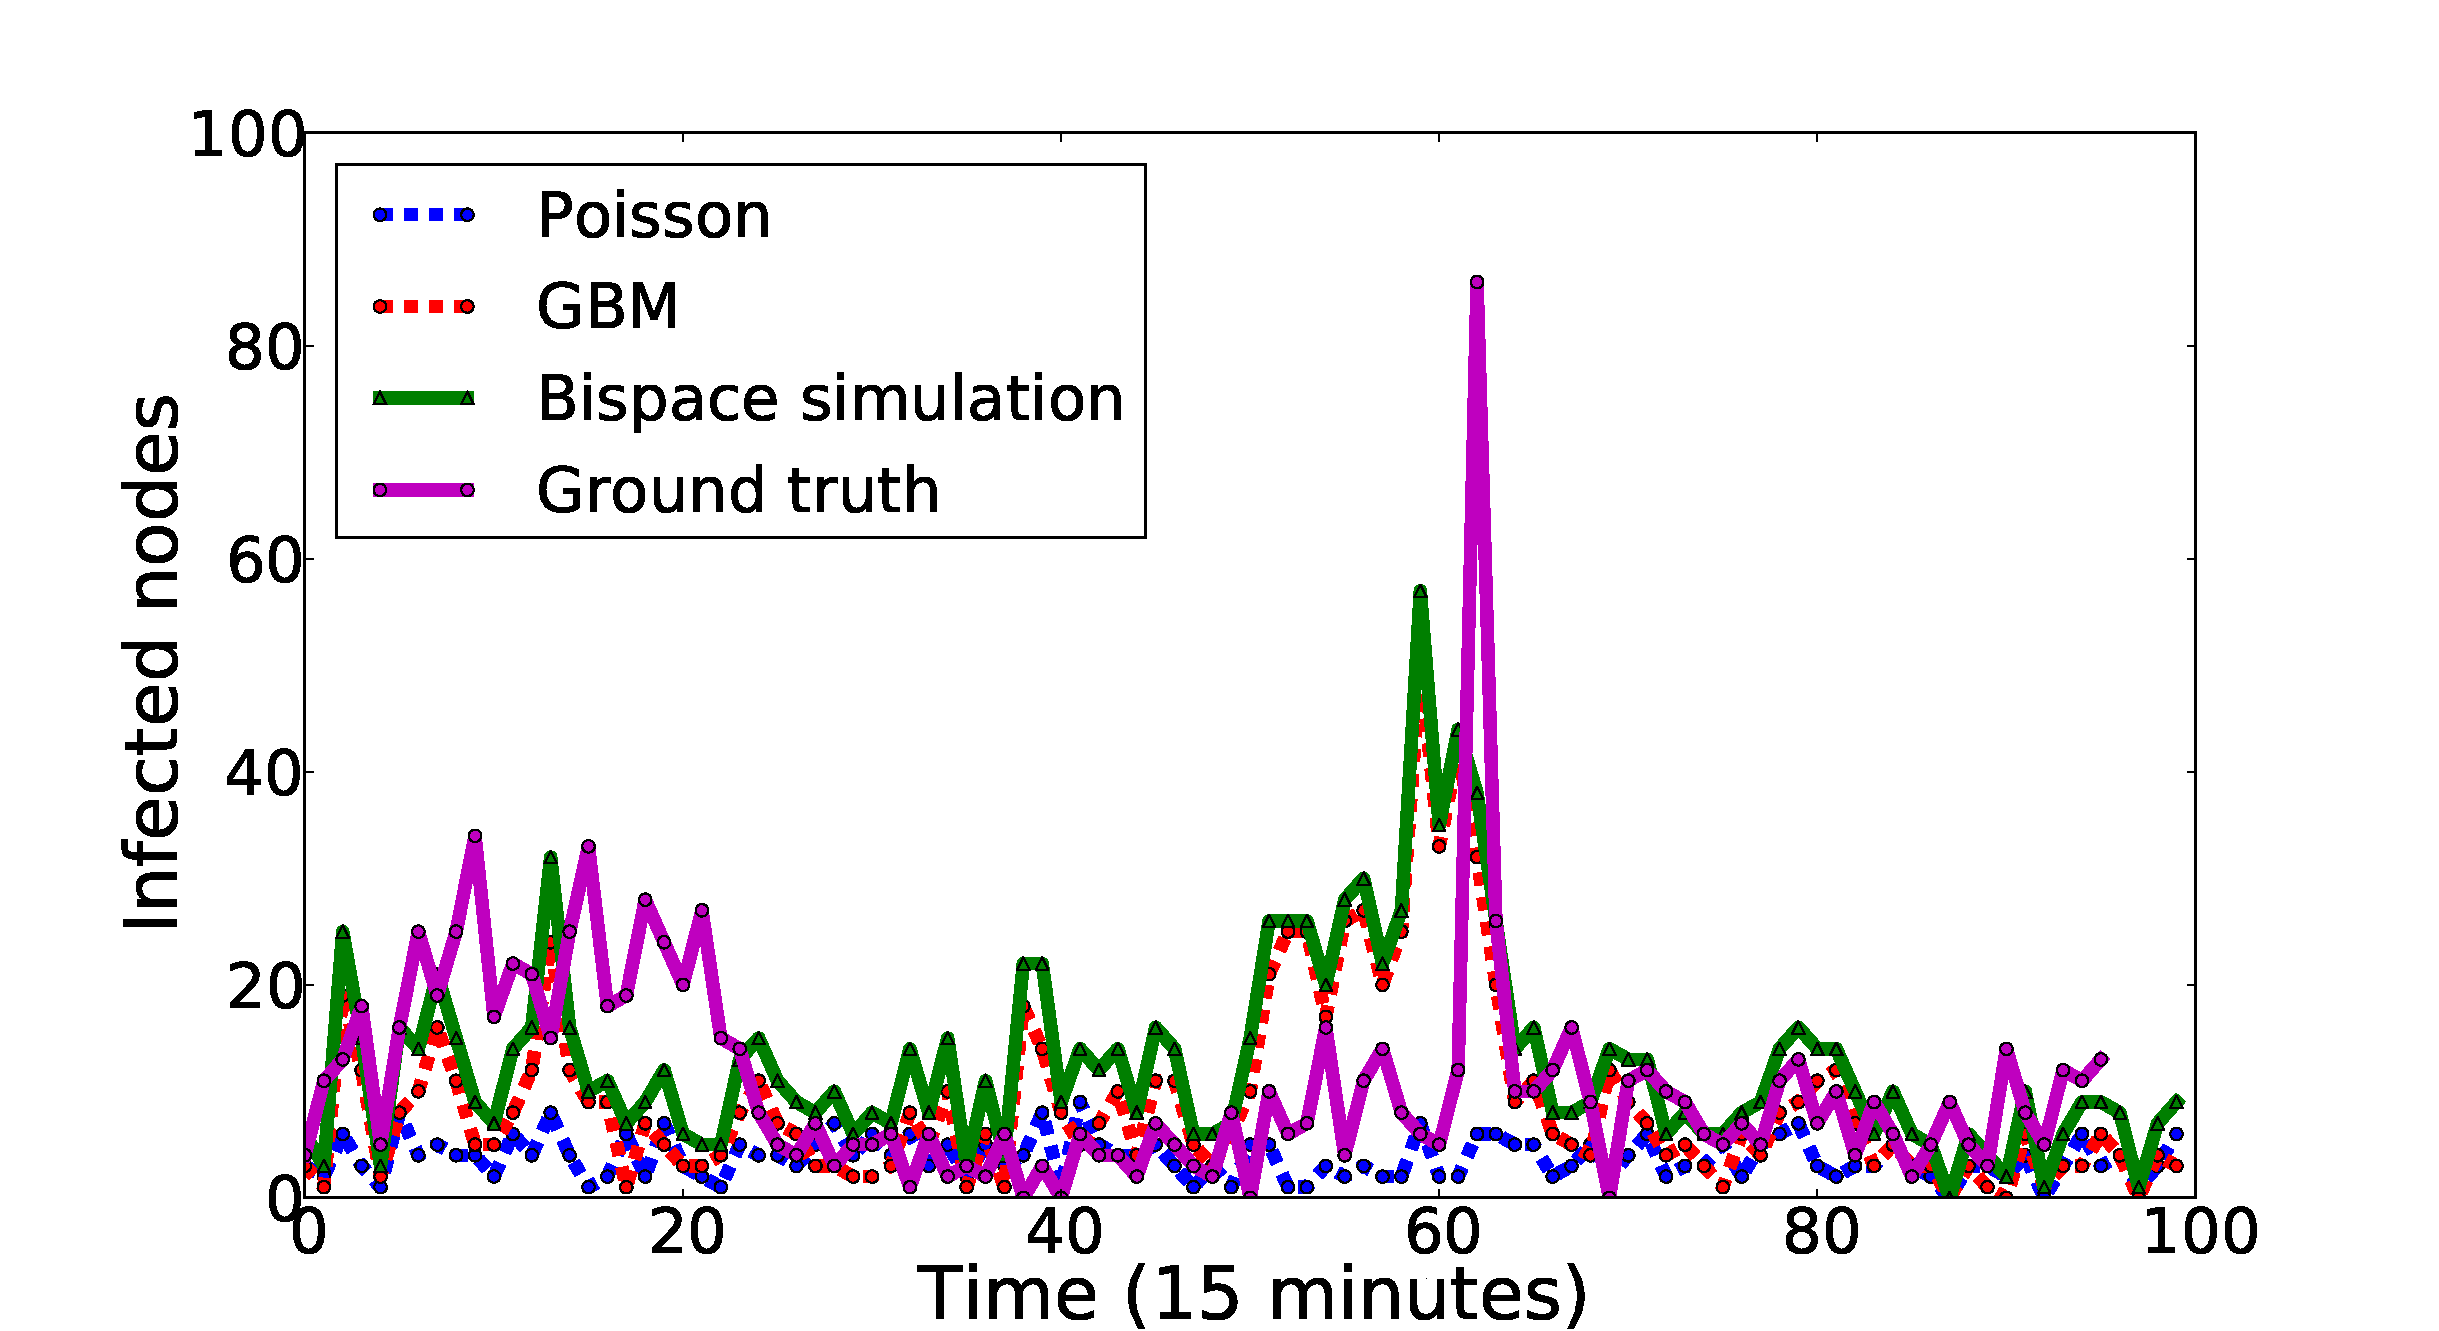
\includegraphics[width=3in,height=1.6in] {figures/4-teacher-with-community-final.pdf}
  \label{fig:teacher_community}
 }
\caption{GBM and Poisson propagation simulation for teacher protests (Mexico)
on Sep 1, 2013.}
\label{fig:4teacherSimulation}
\end{figure}


\begin{figure}[th]
\centering
\subfigure[Simulation without community]{
   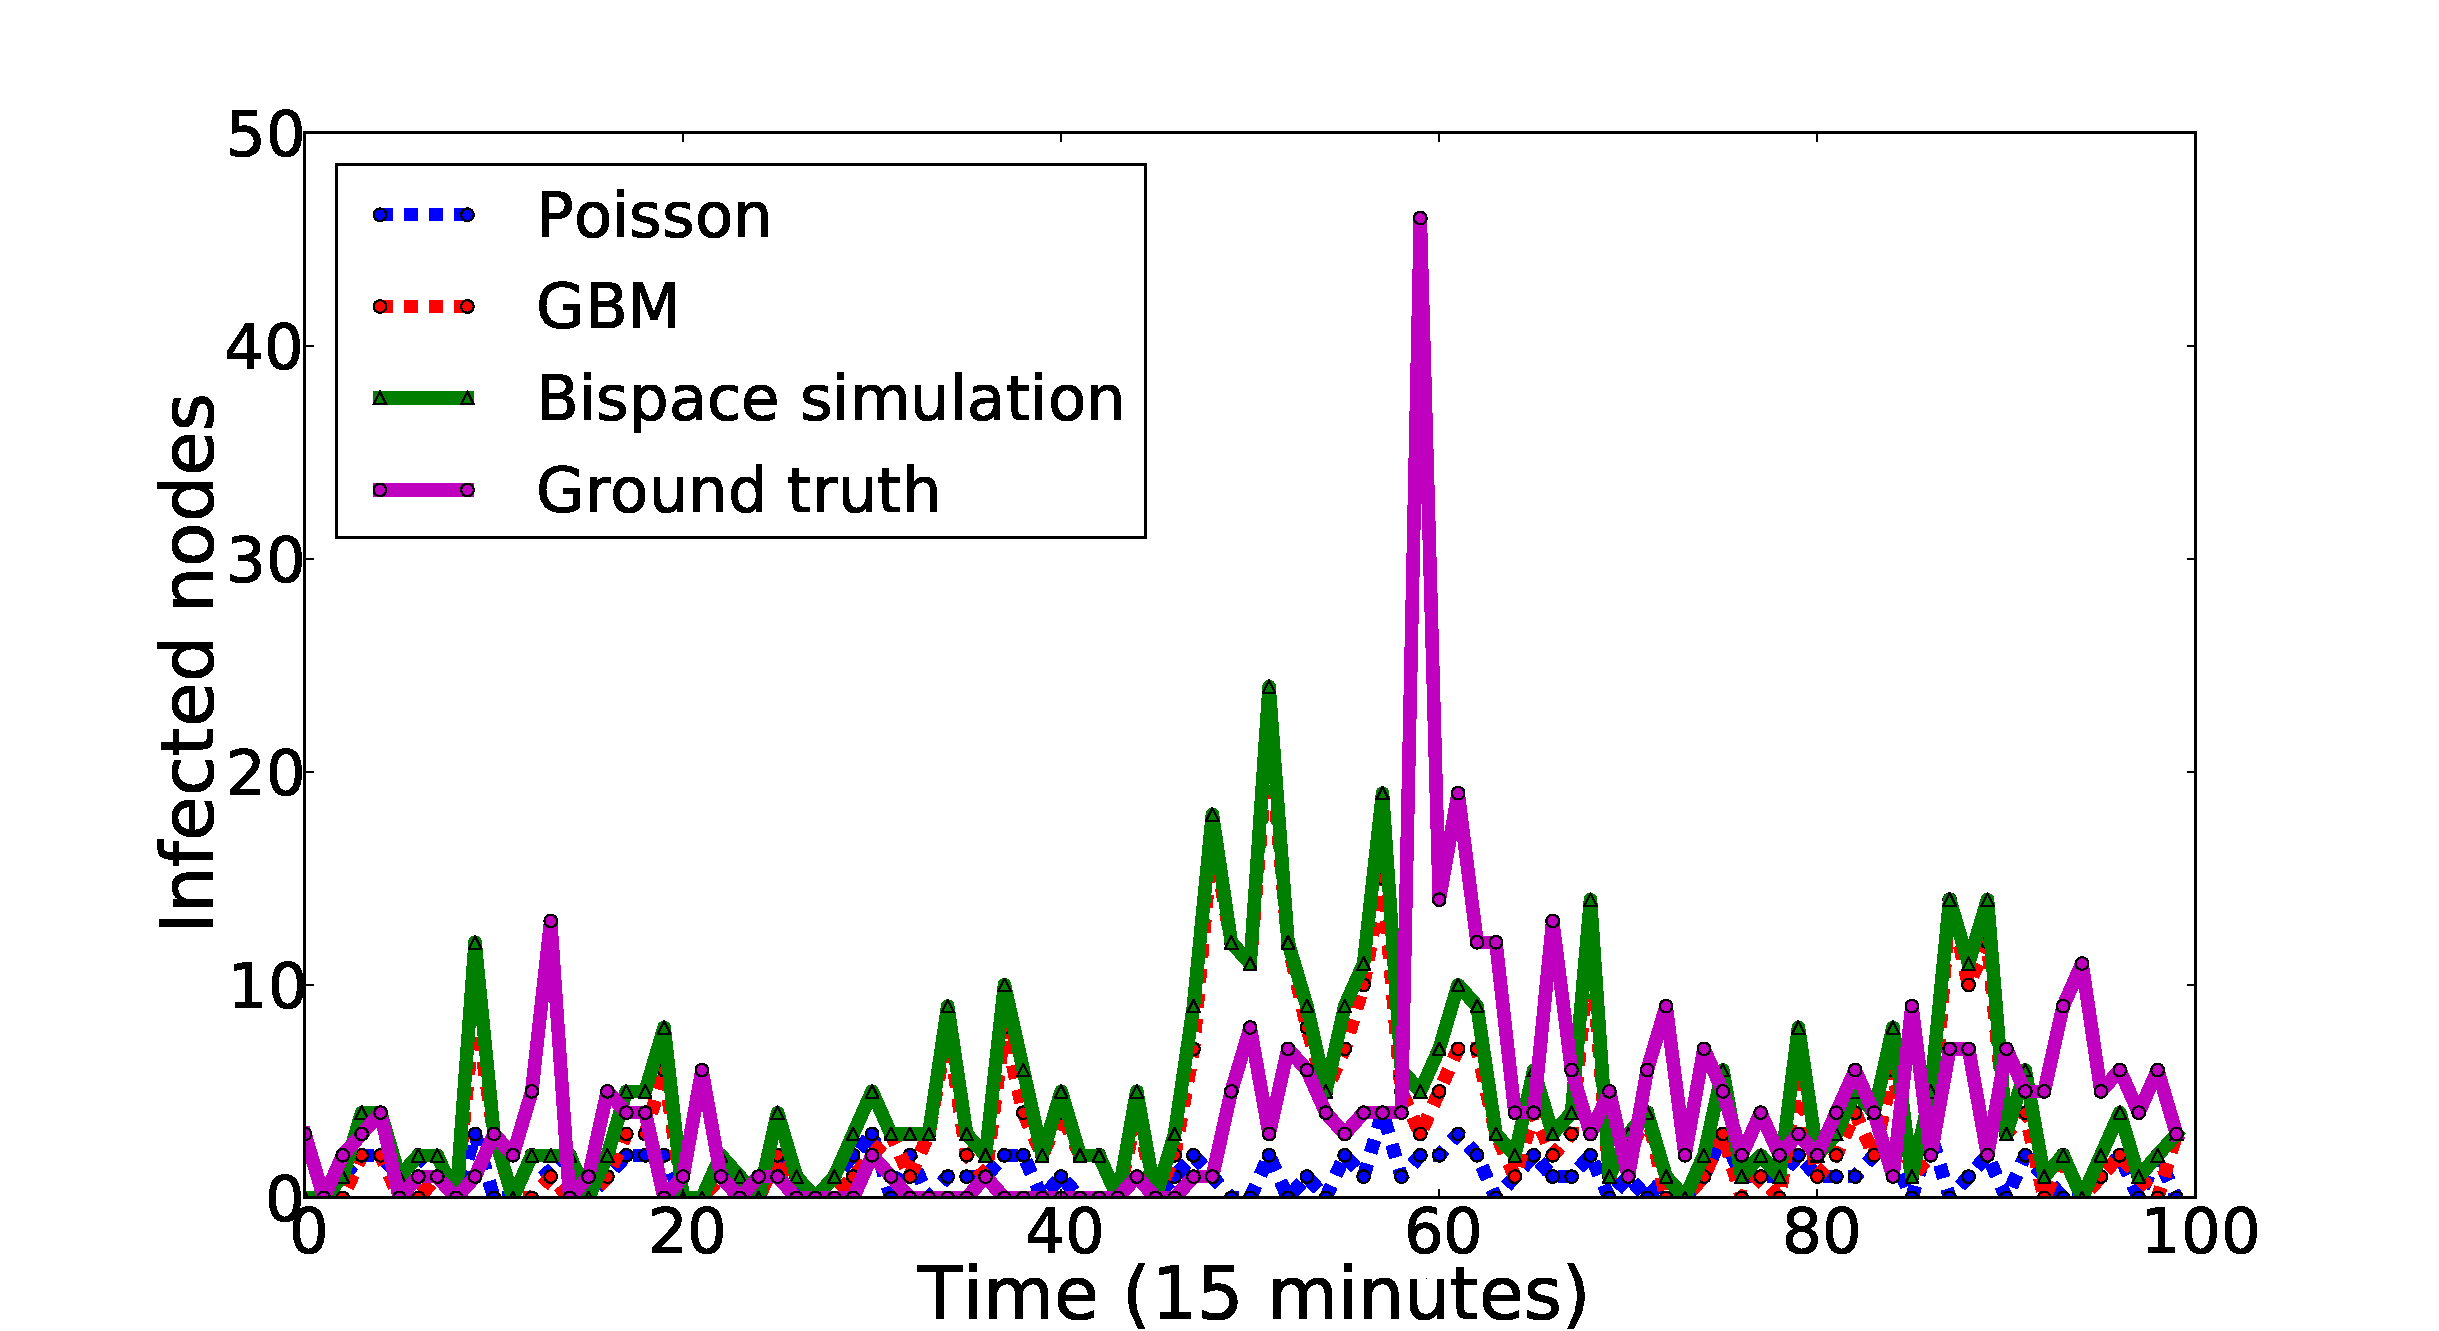
\includegraphics[width=3in,height=1.6in] {figures/7-colombia-without-community-final.pdf}
  \label{fig:colombia_no_community}
 }
 \subfigure[Simulation with community]{
   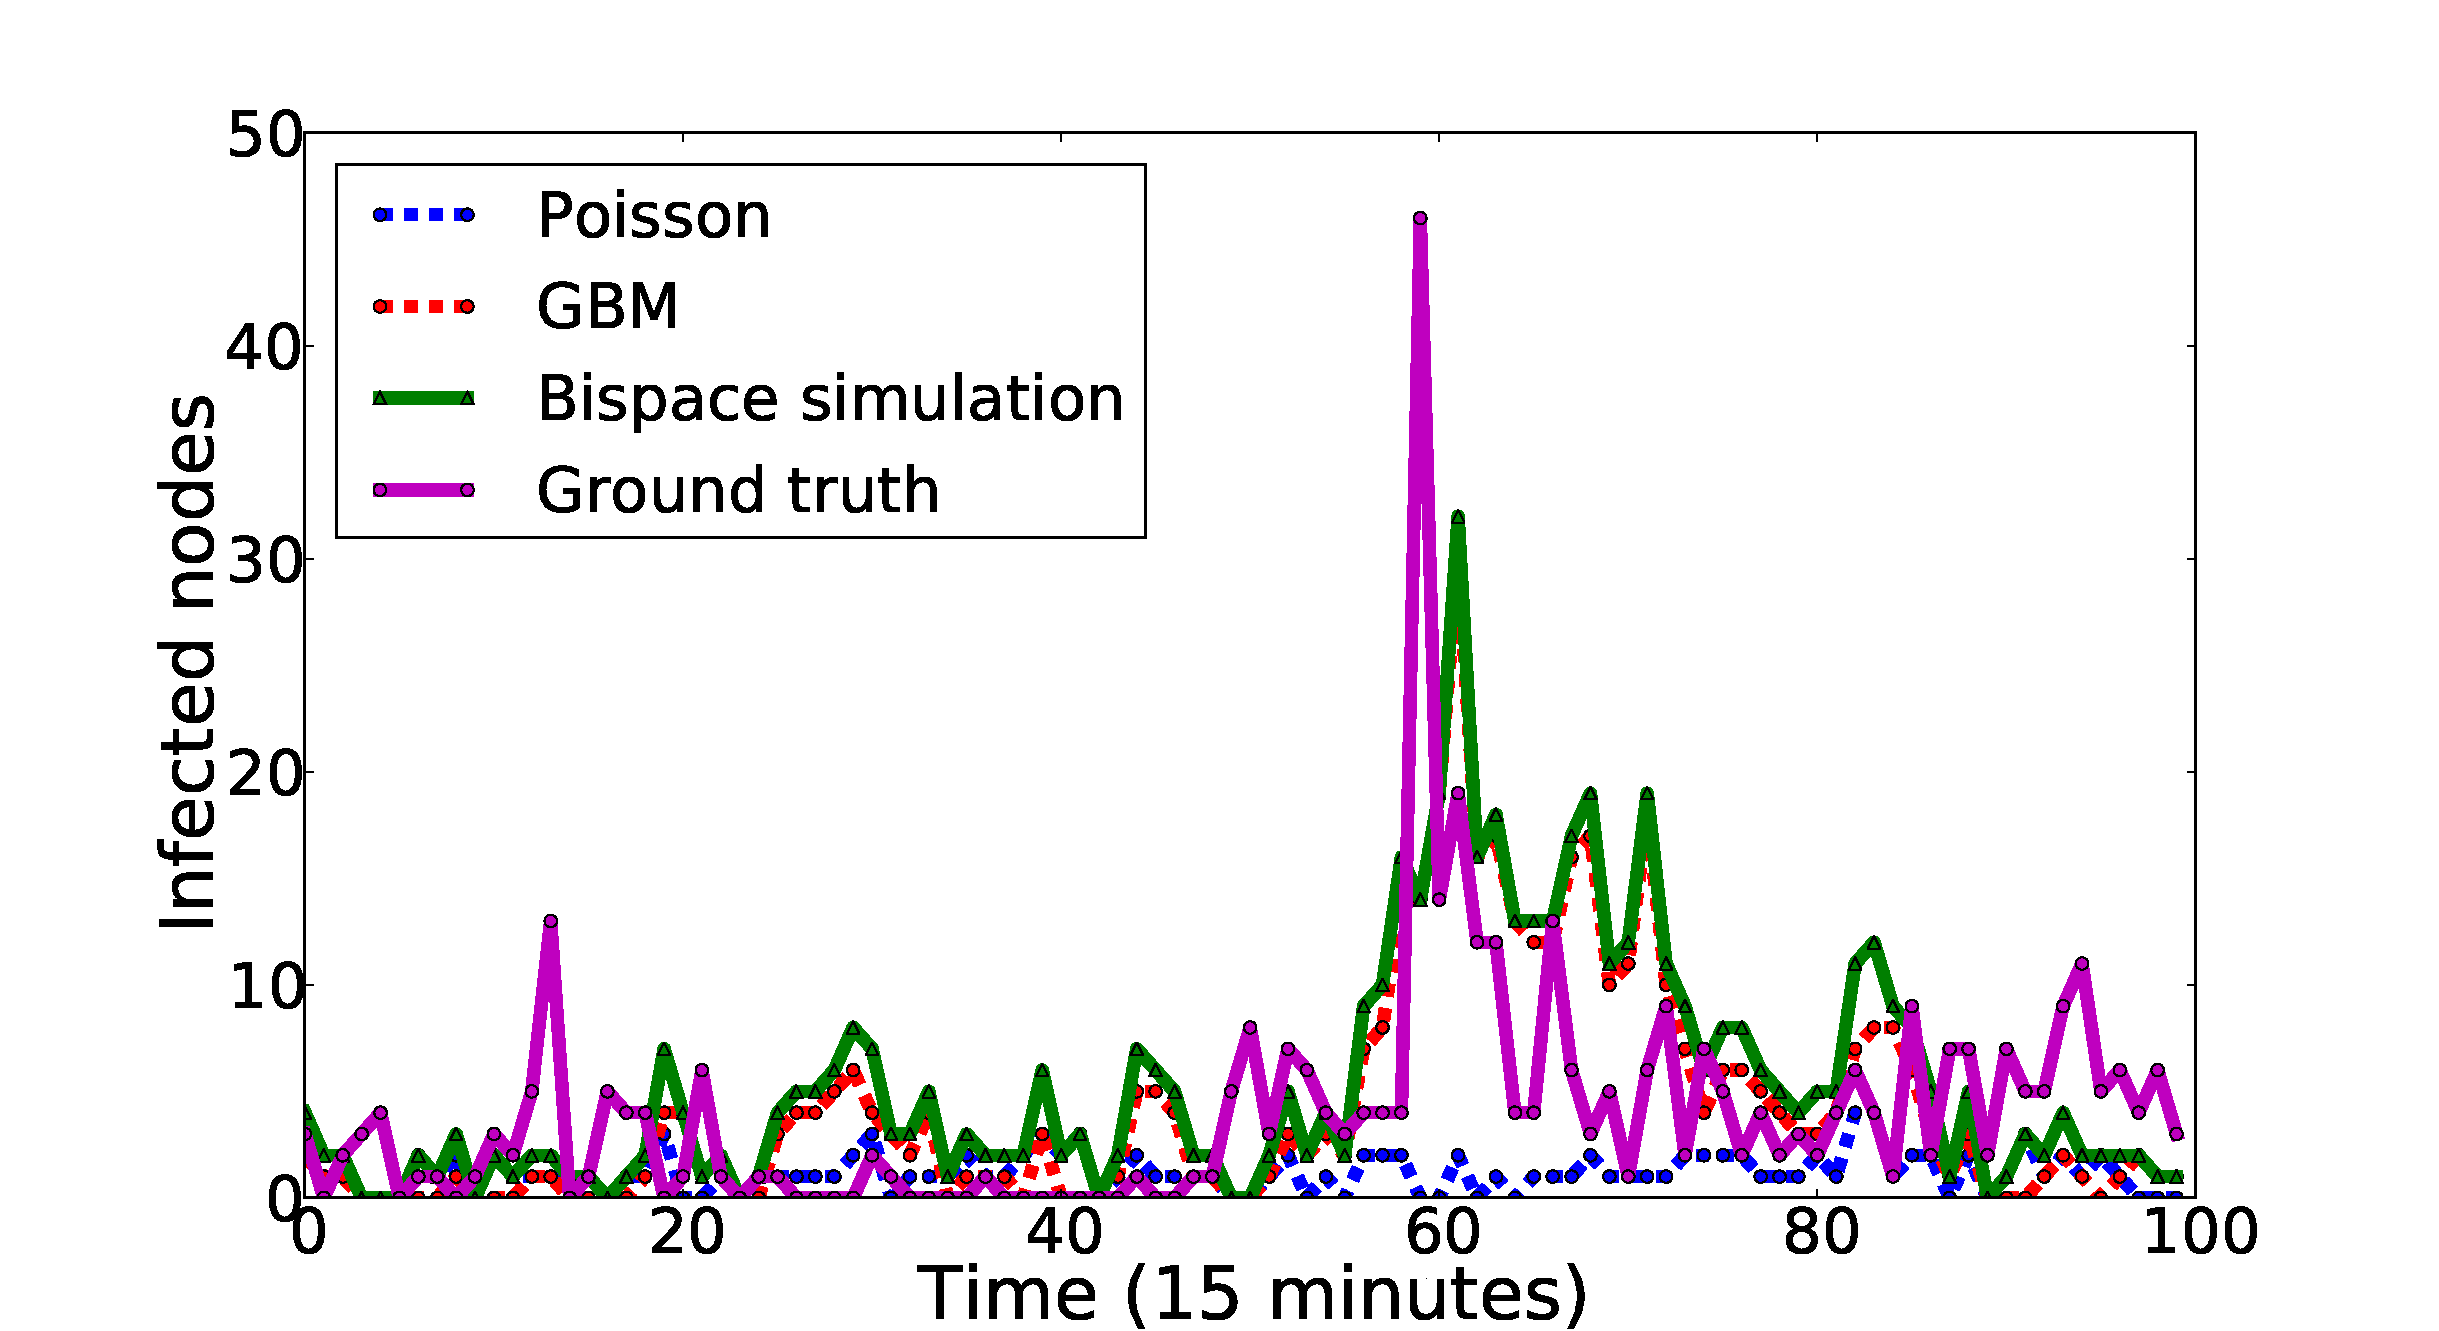
\includegraphics[width=3in,height=1.6in] {figures/7-colombia-with-community-final.pdf}
  \label{fig:colombia_community}
 }
\caption{GBM and Poisson propagation simulation for Colombia protests on Dec 4, 2012.}
\label{fig:7ColombiaProtest}
\end{figure}




\subsection{GBM Diffusion Model}
For each of our mass protest events, we filter by its specific keywords (hashtags) to obtain a set of relevant tweets and construct a mentions network from those tweets. We assume that information propagates from an initial infected user to other users through the network from one node to its neighbors. We build an adjacency matrix based on the mentions network and simulate the propagation using the GBM diffusion process as follows:
\begin{enumerate}
  \item \textbf{Brownian distance:} The Brownian distance is intended to have
an inverse relationship with mention frequency. As Fig.~\ref{fig:timecurve} shows, users with smaller Brownian distance have greater mention frequencies resulting in shorter mean propagation times with less variance. From Fig.~\ref{fig:timecurve}, we can see that infection time and variance generally both increase with an increase in Brownian distance. Heuristically, more frequent mentions indicate stronger ties which leads to easier adoption of information.

  \item \textbf{Propagation speed: } To evaluate our dynamic GBM
infection process assumptions, we estimate the GBM parameters for different protest events and depict the GBM propagation curves in Figs.~\ref{fig:1Yosoy2012may},~\ref{fig:4teacherSimulation}, and~\ref{fig:7ColombiaProtest}. The blue curve depicts the Poisson propagation in latent space. The red curve depicts GBM propagation through the mentions network. The green curve is the overall simulation result while the magenta curve depicts the ground truth of the protest events process. By comparing the green and magenta curves, we can evaluate the
effectiveness of our bispace model in simulating the mass protest events.
As shown, we find that, given a mentions network, our bispace model can simulate the propagation speed at a reasonable scale, at the right magnitudes. As seen in Figs.~\ref{fig:yosou_no_community},~\ref{fig:teacher_no_community} and~\ref{fig:colombia_no_community},
we find that we can capture the burst of activity at the same time point as the ground truth during protest propagation.


\end{enumerate}



\begin{figure}[ht]
\centering
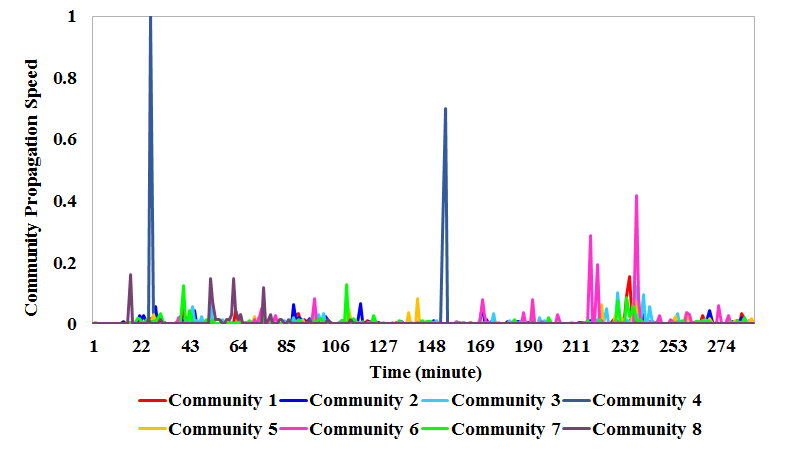
\includegraphics[width=4in] {figures/4teacher-community-speed.png}
\caption{Normalized mass-protest propagation speed for major communities during teacher protest events.}
\label{fig:teacher_community_speed}
\end{figure}



\subsection{GBM Diffusion with Communities}
We were also able to observe the variation in $\mu$ and $\sigma$ as community structure varies. In particular, community features like graph density and diameter as shown earlier in Fig.~\ref{fig:teacher_community_parameters0} may impact GBM propagation.
%To illustrate the relationship between the GBM parameter $\mu$ and graph structure, we plot $\mu$ against diameter and density for several communities in Figure~\ref{fig:density_diameter}. We can see the larger of a community diameter, the higher of propagation parameter $\mu$, while the smaller of graph density, the higher of propagation parameter $\mu$.
We experimented with two modeling approaches: (i) one set of parameters for the whole network and (ii)
different parameters
for each community in the network.
We ran simulations for both these situations,
and plotted the results of the whole network vs. community-specific approach in Figs.~\ref{fig:1Yosoy2012may},~\ref{fig:4teacherSimulation}, and~\ref{fig:7ColombiaProtest}.
Comparing these simulation results, we find the community approach performs better, especially at capturing peak values. Taking a closer look at Fig.~\ref{fig:teacher_community_speed}, we observe that propagation time and speed of infection are different for each community and we are able to simulate local propagation more accurately, which can be seen, e.g.,
from Fig.~\ref{fig:teacher_community}, where
the GBM with community method can simulate the burst
propagation effectively, while the general GBM method (see Fig.~\ref{fig:teacher_no_community}) fails to capture the exact peak time.


\begin{figure}[ht]
\centering
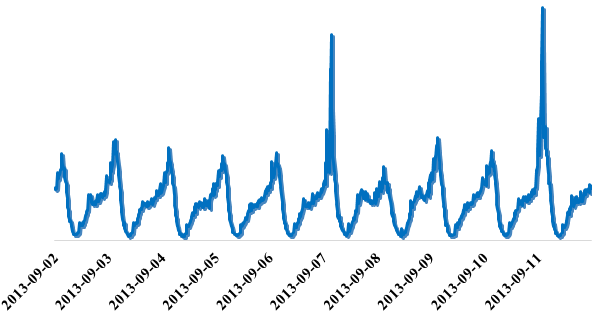
\includegraphics[width=3.2in, height=1.9in] {figures/Baseline.png}
\caption{Total tweets over time from Sep 2 to Sep 11, 2013 (Mexico).}
\label{fig:Baseline}
\end{figure}

\subsection{Latent Space Diffusion Model}
We use the following steps to calculate the properties of the latent space for each event.

\begin{enumerate}
  \item \textbf{Latent space:} The intent is
to consider all possible external influences and latent interactions in this space. We split Twitter data into unique 15 minute intervals and count the total
number of infected users in each interval.
  \item \textbf{Normalize:} Twitter user activity varies based on time of day and day of week (see Fig.~\ref{fig:Baseline}). For each 15 minute window from Step 1, we find the average number of tweets over a 4 week period and use this value to normalize the count. This baseline count of tweets over time in the latent space is close to the Poisson distribution.
  Fig.~\ref{fig:Poisson_Sep3} shows an example of this baseline.
  \item \textbf{Train: } Using one week's data split into 15 minute intervals, we train the Poisson distribution parameters.
  Fig.~\ref{fig:poissonianCurve} shows that the training curve and ground truth curve can be matched quite well.
\end{enumerate}


\section{Evaluation results}

\begin{table*}[!ht]
\tiny
\caption{GBM simulation results for teacher protest events on Sep 2, 2013.}
\vspace{0.5em}
\centering
\begin{tabular}{|c | c | c | c | p{3cm}<{\centering} | p{2.5cm}<{\centering} | p{2.5cm}<{\centering} |}
\hline
& Average degree & Diameter & Graph density &Connected components& Average clustering coefficient & Average path length  \\ [1ex]
\hline
Simulation& 1.791 & 11&  0.002& 183& 0.083 & 4.786  \\[1ex]
\hline
Ground truth&  1.726 & 18 & 0.002 & 204& 0.008 & 6.261  \\[1ex]
\hline
\end{tabular}
\label{table:simulation_location}
\end{table*}


We present an exhaustive evaluation of our bispace simulation approach
alongside various dimensions next:

\begin{itemize}
  \item \textbf{How effective is the performance of the bispace model?}
\end{itemize}
Recall that
the bispace modeling is comprised of
two independent process: the GBM simulation in the mentions network,
and
the Poisson process within the latent space.
Given an initial mentions
network, after training the GBM parameters of $\mu$ and $\sigma$, we proceed to conduct the GBM simulation. After estimating the Poisson parameter $\lambda$, we are able to do the
Poisson simulation within latent space.
We see that the GBM model
is capable of capturing many mass protest scenarios, to the order of magnitude.
Even though it cannot simulate the propagation speed accurately
at every time point, the method is effective at capturing the total
number of infected nodes with an accuracy of $[0.78,0.95]$, as shown
in Fig.~\ref{fig:GBM_compare_community}.

\begin{itemize}
  \item \textbf{How adept is the bispace
model at capturing surge/burst moments?
How reliable are the simulation results?}
\end{itemize}
Fig.~\ref{fig:1Yosoy2012may} depicts the analsis
of the YoSoy132 student movement, whose Twitter activity is generally tortuous, and the curve is full of surges and bursts. From
Fig.~\ref{fig:1Yosoy2012may} we see that the bispace model is
capable of simulating the general surge trends. Comparing
the bispace simulation results with ground truth, we can see
at many time points, the bispace simulation matches the ground truth.
Fig.~\ref{fig:7ColombiaProtest} shows the second protest of people protesting
against the government in Colombia; here
the Twitter activity depicts a burst at a single time point which is
hard to capture. We can see the bispace model did show there is
a burst, but not at the precise
time point, one of its current limitations.


\begin{itemize}
  \item \textbf{Is the performance of the model better
taking into account community structure?}
\end{itemize}
After numerous experiments, we plot the accuracy distribution of both approaches for all our mass protest situations
in Fig.~\ref{fig:GBM_compare_community}. Although the accuracies are
sometimes interspersed, we can see that in overall
the community model generally has a higher accuracy.

\begin{figure}[ht]
\centering
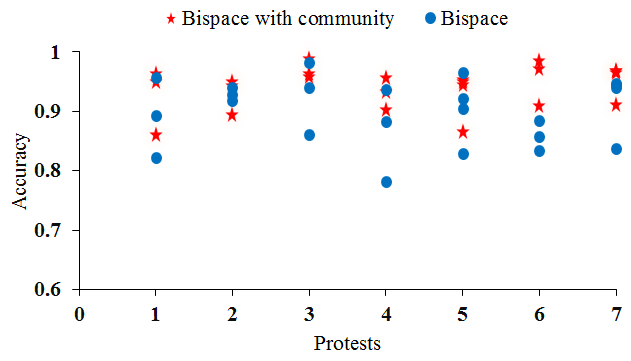
\includegraphics[width=3.3in] {figures/GBM_compare_community.png}
\caption{Performance accuracy of the bispace model for the 7
protest scenarios considered here,
with and without community structure.}
\label{fig:GBM_compare_community}
\end{figure}


\begin{itemize}
  \item \textbf{Can the bispace model simulate the propagation path?}
\end{itemize}
In addition to comparing the simulated counts of tweets over time with ground truth values, we can also compare the propagation path generated by the simulation against the actual propagation path
through the mentions network. In Fig.~\ref{fig:simulation_truth} we can
obtain a sense of the type of infection network bispace modeling creates as
compared with the actual network. The simulation produces networks with relatively accurate paths and relevant characteristics as shown in Table~\ref{table:simulation_location}. The component to which a user belongs is that of neighbors who can be reached from connected paths running along edges of the graph~\cite{newman2003structure}.


\begin{figure}[ht]
\centering
\subfigure[Simulation results]{
   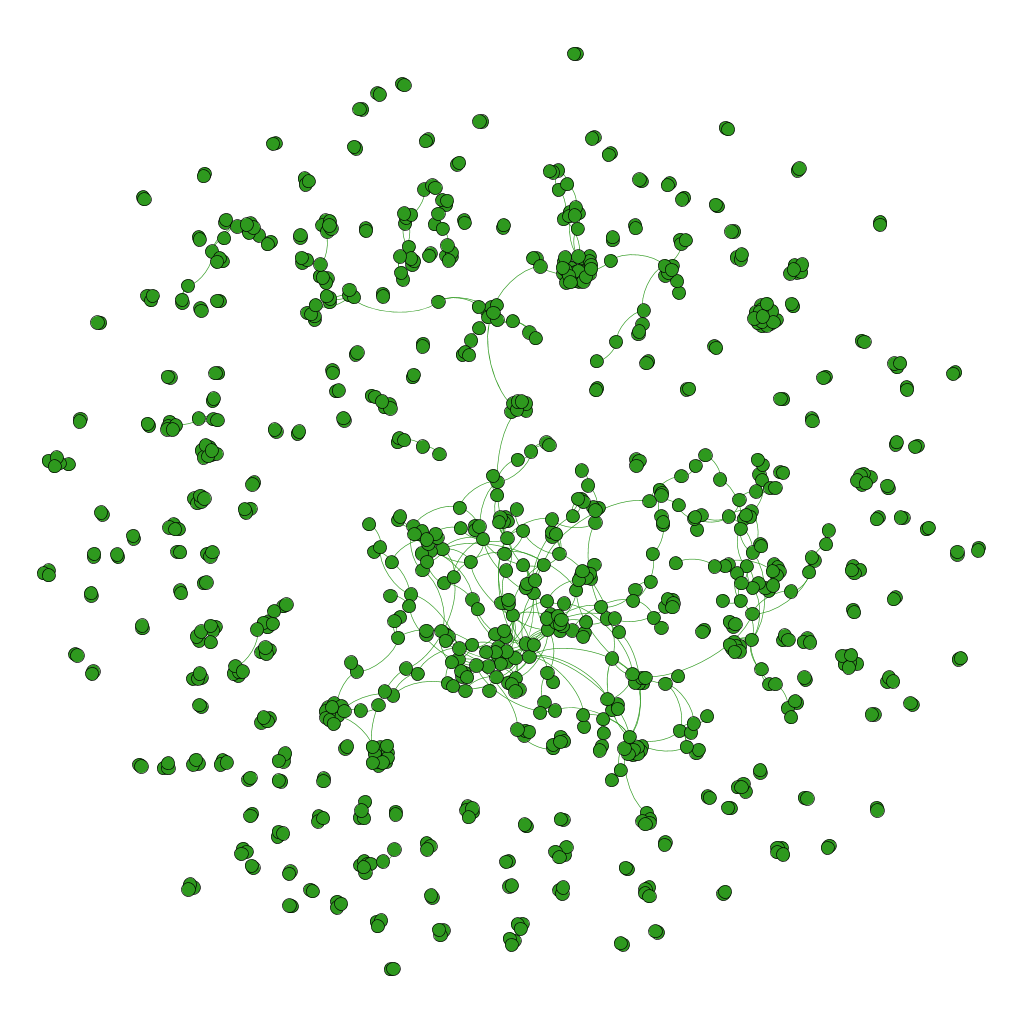
\includegraphics[width=2in, height=2.1in] {figures/evaluation_simulation.png}
  \label{fig:Simulation result}
 }
 \subfigure[Truly infected nodes]{
   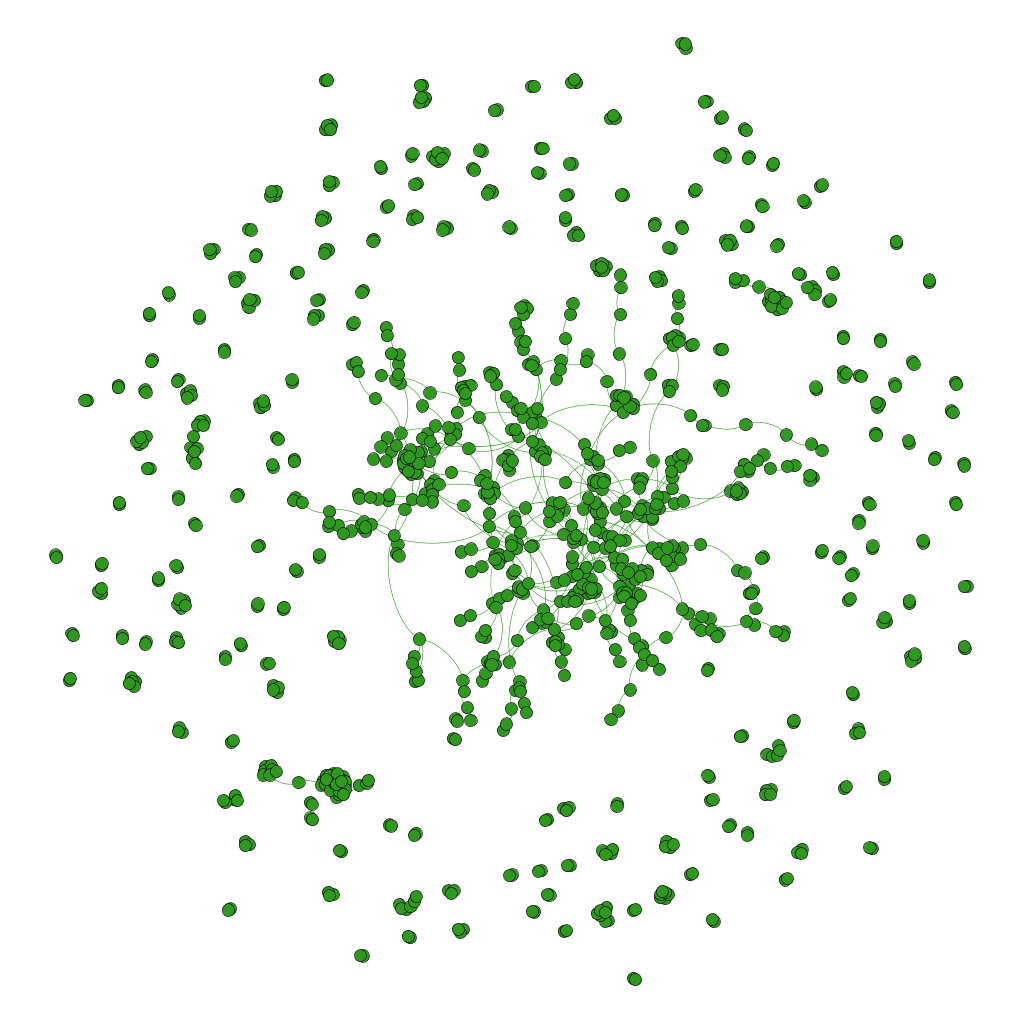
\includegraphics[width=2in, height=2.1in] {figures/true_t_mention_evaluation.png}
  \label{fig:Truly infected nodes}
 }
\caption{Bispace model simulation results compared against
ground truth infected nodes for the Mexican teacher protest events.}
\label{fig:simulation_truth}
\end{figure}




\begin{itemize}
  \item \textbf{Between the geometric Brownian model and Poisson
propagation approaches, which model
is more dominant during the simulation process?}
\end{itemize}
From Figs.~\ref{fig:1Yosoy2012may},~\ref{fig:4teacherSimulation},~\ref{fig:7ColombiaProtest}, by observing the blue dashed line (Poisson) and red dashed line (GBM), we can see that
the Poisson process shows a mild activity, while the GBM model
serves as the dominant component which can capture the moments of key
surges.

%!TEX root = ../main.tex
% mainfile: ../main.tex

\section{Discussion}
In this paper, we have characterized mass protest propagation using a
bispace model comprising an observed mentions network space and a latent space. We have introduced a trust function to simulate propagation in observed space using a geometric Brownian motion diffusion process which can be further extended to support communities with different propagation parameters per community. We
considered the latent space of all interactions outside the mentions network to be a Poisson distribution process. We have shown how the GBM diffusion model offers a new approach for modeling propagation through social networks like Twitter. Through our experiments, we find that the time required for spread of protest information through such networks is dependent on the network's substructures. Furthermore, we find that modeling the diffusion process on a community basis provides better results than the assumption that all nodes in the network spread information in the same way.

In future work, we hope to further characterize the hidden network with the goal of uncovering specific latent variables. Additionally, we envision applying the GBM model to other networks, such as the Twitter follower network, to identify those paths most susceptible to information dissemination. Finally, we desire
to compare propagation of mass protest language against other themes,
such as celebratory events, to aid in determining correlations
between topic or sentiment and the resulting social media diffusion.

%In future work, we hope to further characterize the hidden network to discover latent factors. Additionally, we would like to apply the GBM model to friends networks or other association networks to see which network is more adoptable for propagation paths. Further, we want to compare the mass-protest events propagation with other topics such as celebration events to determine the relevance of topic or sentiment in social media propagation.

%how the community structure constrain or promote the propagation process.
% The other aspect we want to focus on is the change of the properties of the mentions network before and after mass-protest-speech sighting. One of the interesting questions we would like to address is whether people start to counter-mention \textit{mass-protest}. In such cases, one would expect mention-links to be formed between nodes with high geodesic distance.
%We also like to extend the Geometric Brownian motion into dynamic


\endgroup
